\documentclass{article}
\usepackage{setspace}
\usepackage{natbib}
% Language setting
\usepackage{subfig}
\usepackage[english]{babel}
\usepackage{float}
\usepackage{hyperref}

% Set page size and margins
% Replace `letterpaper' with `a4paper' for UK/EU standard size
\usepackage[letterpaper,top=2cm,bottom=2cm,left=3cm,right=3cm,marginparwidth=1.75cm]{geometry}

% Useful packages
\usepackage{amsmath}
\usepackage{graphicx}
% \usepackage[colorlinks=true, allcolors=blue]{hyperref}
% \usepackage{xr}
% \externaldocument{supplementary}





\begin{document}

\begin{titlepage}
   \begin{center}
       \vspace*{2cm}
       \Large

       \textbf{Re-analysis of Variant Effect Maps}

       \vspace{0.5cm}
        BCB330 Final Report
            
       \vspace{1.5cm}

       by \\
       \vspace{1.5cm }

       Bilin Nong

       \vspace{4cm}

        Supervisors: Jochen Weile \& Fritz Roth
    
           \vspace{6.5cm}  
     

       University of Toronto\\
       
       \today
        
       \vspace{0.8cm}
            
   \end{center}
\end{titlepage}

% double-space
\setstretch{2}
\large
\section{Introduction} % 3 pages
The interpretation of clinical variants is a difficult process. To classify variant effects, the American College of Medical Genetics and Genomics (ACMG) guidelines\cite{richards_standards_2015} provides  categories ranging from "pathogenic" to "benign", with uncertain cases labeled as "variants of uncertain significance" (VUS), where insufficient evidence exists. The majority of clinical variants are currently classified as the latter\cite{weile_multiplexed_2018}. The ACMG guidelines assign different evidence strengths to different types of information, such as \textit{in silico} predictors or laboratory studies. Unfortunately, while computational predictions are easily scalable, they are only considered "supporting" evidence, whereas the stronger evidence provided by laboratory assays traditionally only exists at small scale.

\subsection{MAVE: Multiplex Assays of Variant Effect}
To tackle the problem of scaling laboratory assays, a proactive approach called Multiplexed Assays of Variant Effect (MAVEs)\cite{Starita295279} was developed. MAVEs harness high-throughput sequencing to apply laboratory assays at scale and often also integrate machine learning methods and clinical expertise.
MAVE studies typically include four main steps: mutagenesis, selection of variants via assay, sequencing, and computational analysis. A good example for a mutagenesis method is Precision Oligo-Pool based Code Alteration(POPCode) mutagenesis, which aims to yield a complete spectrum of possible amino acid changes across the protein \cite{weile_framework_2017}. Following mutagenesis, the resulting variant libraries are subjected to a selection step, enriching or depleting variants based on their effects on protein functionality. There are many selection schemes that can be applied in a MAVE, such as functional complementation, Yeast-2-Hybrid (Y2H) assays, or sorting based on fluorescent reporter activity via FACS (fluorescence-activated cell sorting). Sequencing is then used to quantify the enrichment or depletion of variants as a result of selection. There are different sequencing approaches including Tileseq\footnote{\url{https://github.com/rothlab/tileseqMave}} and Barseq\footnote{\url{https://github.com/rothlab/pacybara}} which can be used in this step.
The last step in MAVE is computational analysis, where pipelines and scripts are employed to analyze the sequencing readout and calculate the selection advantage for each variant.

Nowadays, MAVEs generate lots of variant effect maps of clinically relevant genes for clinical research. However, there are some issues related to MAVEs. First, going from MAVEs to clinical interpretation is not straightforward, since the selection advantage for each variant in a given assay may not reflect their pathogenicity. For this reason, including a Log-likelihood Ratio (LLR) approach in the downstream analysis of MAVEs has been proposed. This approach can transform the fitness scores into a metric of evidence strength towards or against pathogenicity of variants. Second, computational analysis pipelines have undergone many iterations of developments. Different versions of MAVEs may adopt different implementations, leading to varying outcomes. Therefore, it is important to analyze different versions of MAVEs and evaluate their performance systematically.

\subsection{Goals and Objectives}
Based on the above issues with MAVEs, this BCB330 project aims to re-evaluate the performance of variant effect maps based on different versions of MAVE pipelines with respect to precision and sensitivity on reliable benchmarks.

%Maybe re-state the bullet points from the first report here
\begin{enumerate}
    \item Re-process the raw data underlying existing variant effect maps with the latest versions of their respective analysis pipelines.
    \begin{enumerate}
        \item Inspect the QC outputs for the maps to identify potential quality issues.
    \end{enumerate}
    \item Compile benchmark sets of variants with known pathogenicity from online databases and literature for each map.
    \begin{enumerate}
        \item Explore alternative reference sets of non-disease genes.
    \end{enumerate}
    %The above two goals may also be deserving of sub-objectives
    \item Compare the predictions made by different versions of variant effect maps using the benchmark sets and use them to infer evidence strength for clinical interpretation.
    \begin{enumerate}
        \item Identify disagreeing variant effect outputs, and establish their computational provenance.
        \item Produce Precision-Recall Curves to evaluate the performance of updated version and old version of MAVEs.
        \item Calculate Log-likelihood Ratio transformations and identify the fitness score intervals that corresponding to different evidence levels towards "pathogenic" and "benign" classifications. 
    \end{enumerate}
    \item Provide recommendations for optimizing the implementation of MAVEs based on the evaluation result.
\end{enumerate}

\section{Methods} % 3 pages
\subsection{Reprocessing Maps} 
To re-process the raw data sets using various versions of MAVEs, we use the TileSeqPro pipeline, which takes the raw sequencing output from a Tileseq MAVE experiment, applies quality filters and error corrections, calculates fitness scores, and generates diagnostic Quality-Control plots.

% There are two main components in the TileSeq workflow: \href{https://github.com/rothlab/tileseq_mutcount}{TileseqMut} and \href{https://github.com/rothlab/tileseqMave}{TileSeqMave}. 
% To begin, TileSeqMut aligns the sequencing reads to the reference sequence and uses a Bayesian method to call the most likely true variants. Following this, TileSeqMave, the second component of the TileSeq pipeline, analyzes the variant calling result obtained from the previous steps. It starts by translating variant calls into amino acid changes at the protein-level.  Next, it calculates the enrichment ratios, $log(\phi)$, i.e. the log-ratio between pre- and post-selection frequencies for each given variant and performs error-modeling and quality filtering. Lastly, the "scaleScore" step re-scales the $\log(\phi)$ scores relative to pivot points which represent typical nonsense and synonymous variants. As a result, the final scores are distributed such that 0 represents full loss of function, while 1 represents wildtype-like fitness. The pipeline also includes two QC steps, which generates a series of diagnostic plots.
%Before discussing the differences, you might need a sentence that establishes context for the old pipeline, e.g:
TileSeqPro improves upon an older ``Legacy'' TileSeq pipeline that was employed in the Roth Lab until recently.
There are many difference of implementations between TileSeqPro and the Legacy computational pipelines. Most importantly, the Legacy pipeline collapsed the equivalent codon changes early into amino acid changes, before filtering. While this meant that lower quality data could get past the filters, and error correction could not be performed at nucleotide levels, it had the advantage of boosting the number of reads supporting each data point. In contrast, TileSeqPro calculates functional scores for individual codon changes separately, filters out low quality variants based on a number of different criteria such as the low read count (below a certain threshold), and finally combined them into amino acid changes. Thus, TileSeqPro sacrifices data to avoid systematic error, but as a result may potentially suffer from more noise.  


%Maybe here's a good spot to explain the diffences to the "old" pipeline. I.e. primarily that variant counts were collapsed early by amino acid change, before filtering. While this meant that lower quality data could get past the filters, and biases could not be corrected at nucleotide-level, it had the advantage of boosting the number of reads supporting each datapoint (at the expense of accepting lower quality inputs).



\subsection{Evaluation approaches} 
\subsubsection{Precision-Recall Curve}

There are multiple methods available to assess classification performance, including the Precision-Recall Curve (PRC), Receiver-operator characteristic (ROC)\cite{doi:10.1161/CIRCULATIONAHA.105.594929}, Matthew's correlation coefficient (MCC)\cite{chicco2020advantages}, and F-scores\cite{hicks_evaluation_2022}. However, when evaluating different maps, the PRC stands out as the most suitable approach due to its ability to handle class imbalance, a common occurrence in maps where reference set sizes vary. To further alleviate potential biases, a prior-balancing approach\cite{wu_improved_2021} is used to compensate for differences in reference set sizes. 
To compare the predictions made by the old and updated versions of MAVE, the precision-recall curve (PRC) serves as a straightforward and informative visualization tool.  Precision is defined as the fraction of true positive calls out of all positive calls, or in the context of variant effects, the proportion of correctly predicted pathogenic variants out of all predicted pathogenic variants. On the other hand, recall represents the fraction of true positive calls out of all actual cases, or in the context of variant effects, the fraction of variants correctly identified as pathogenic among all existing pathogenic variants.\cite{james_introduction_2021} 
%Better cite a statistics textbook here instead of our framework paper. %I moved the definitions here as it seemed to flow better.

Utilizing the PRC offers numerous advantages in evaluating the performance of these prediction maps.  First, since high precision is crucial in the context of clinical decision based on prediction, we can compare the recall level of these maps under the threshold of 90\% precision: the precision-recall curve provides a numerical values (REC90) describing this information. Second, an overall assessment can be made by analyzing the total area under the curve (AUPRC), which provides a summary measurement of the precision-recall curve. 

\subsubsection{Compiling Benchmark Sets} 
%best to exlain this in the context of PRC curves maybe, as the
To evaluate variant effect maps via Precision-Recall curves, we require adequate reference sets of know pathogenic and benign benchmark variants. To generate such reference sets, we use a script that is built into TileseqPro, which offers automated generation of benchmark sets tailored to specific disease-causing genes, drawing from reliable sources such as
ClinVar\cite{10.1093/nar/gkx1153} and gnomAD\cite{Chen2022.03.20.485034} controls.
Since ClinVar tends to contain more pathogenic variants than benign, gnomAD is used for supplementing the benign variants collect at population level.
The script provides options that allows users to define specific criteria, including allele frequency threshold, quality, and trait of interest. These features allows for the refinement of reference sets, which enhances their applicability in the downstream analysis, includes drawing precision-recall curve, and finding transformation functions from fitness scores to the log-likelihood ratio for pathogenicity. At the same time, there exists some limitations when using gnomAD and ClinVar as reference sources. First, there can be variations in the reliability of ClinVar submissions, since ClinVar collects submissons of interpretation with varying standards of provenance, and some submissions might lack detailed evidence. Second,  variants in gnomAD controls can only serve as a proxy-benign set, as they have not been officially classified. Finally, the validation of maps for non-disease genes will require alternative approaches, such as comparison against high-quality computational predictors.
% You may want to explain why gnomAD controls are used to supplement ClinVar data and the limitations of this approach. What are the limitations of this? (e.g. reliability of ClinVar submissions, validity of using gnomAD controls as quasi-benign benchmarks, evaluating maps for non-disease genes) What to do when automated approach yields no good results? (Manual curation?)


%Another thing to discuss here is that you might want to inspect the QC outputs for the maps to identify any quality issues and compile them in reports.

\subsubsection{Correlation against computational predictors}
%Discuss here how you compared maps against VARITY 
To compare the performance of TileseqPro and the Legacy Tileseq pipelines from another perspective, we did the moving window correlation analysis between Tileseq scores versus VARITY\cite{wu_improved_2021} scores along amino acid positions. VARITY is a computational method for pathogenicity prediction, it provides a probability of pathogenicity scores by harnessing gradiant boosted trees algorithm to weight input training sets, where more close to 1 for variants that are inferred to be pathogenic, and more close to 0 for variants that are inferred to be benign. 
%Also definitely explain the difference between VARITY_R and VARITY_ER here, since it's referenced later in the results section!

There are two VARITY models generated by the VARITY framework: VARITY\_R and VARITY\_ER. The VARITY\_R model included rare ClinVar\cite{10.1093/nar/gkx1153} variants with global minor allele frequency (MAF) less than 0.5\% in its core training/ test set; while VARITY\_ER model only included extremely rare ClinVar variants with MAF less than ${10}^{-6}$ in its core set. The score scale of VARITY is completely opposite to which of the fitness score produced by Tileseq pipelines, therefore, we measured the performance of fitness scores by comparing their anti-correlation with VARITY scores.


\subsubsection{Log-likelihood Ratio of Pathogenicity}

In the context of pathogenicity assessment, the log-likelihood ratio (LLR) for pathogenicity\cite{weile_shifting_2021} can be used to evaluate the likelihood of a variant being pathogenic versus benign based on the data. While we can get the fitness scores of the variants from the maps, these scores only represent the effect of variants on protein function, and they do not necessarily reflect pathogenicity (i.e. how likely they will cause diseases)\cite{floyd_proactive_2023}. We first estimate the probability densities across the scores of pathogenic and benign reference variants, respectively, via kernel density estimation. The log ratio between the density functions is then used to calculate the LLR of pathogenicity, expressing how much more likely a variant at a fitness score is to be pathogenic than it is benign\cite{floyd_proactive_2023}. However, this method is very sensitive to even small differences in metaparameter choice, particularly kernel bandwidth and requires careful manual supervision.

%May be worth explaining why we don't see high LLRs for scores near 0 (contrary to expectation). Absence of reference variants in those regions may be explained by dominant-negative inheritance pattern for Calmodulin.

\section{Results}
\subsection{SUMO1}
%Some intro here, e.g.
We first re-calculated the map for SUMO1, one of the first variant effect maps created in the Roth Lab\cite{weile_framework_2017}.
\subsubsection{Observations from QC results}

Examining the distributions of synonymous and nonsense variant enrichment ratios ($\log(\phi)$) relative to marginal frequency (see supplemental Fig. 1) reveals an acceptable separation between the two at a frequency of $10^{-4}$. Given the sequencing depth of 1.5M reads per sample, this suggests an ideal cutoff of 150 reads. After setting filters accordingly, approximately one in three variants were filtered out by the frequency filter and bottleneck filters.

% \begin{figure}[H]%
%     \centering
%     \subfloat[\centering the $log(\phi)$ bias plot]{{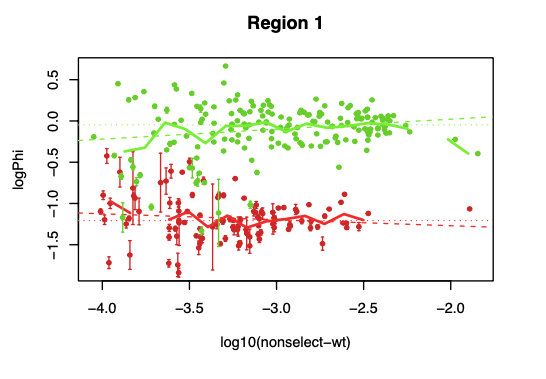
\includegraphics[width=.45\textwidth]{Figures/SUMO1/logphi_bias.png} }}%
%     \qquad
%     \subfloat[\centering filtering breakdown]{{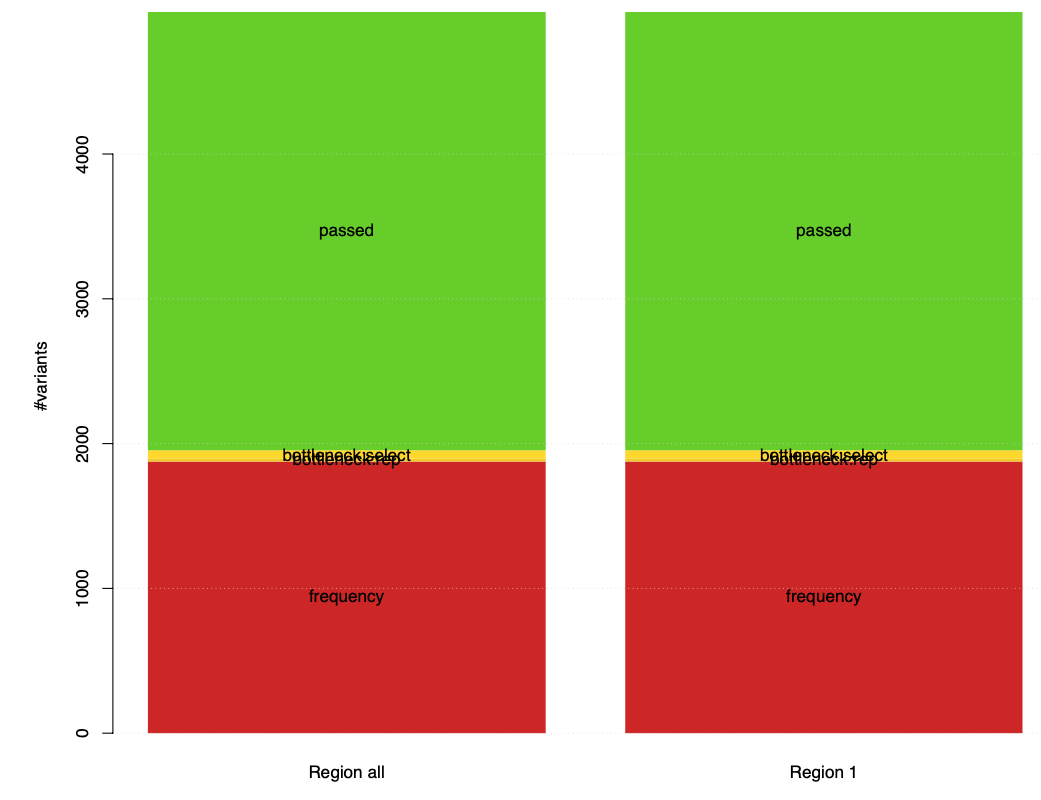
\includegraphics[width=.45\textwidth]{Figures/SUMO1/filtering.png} }}%
%     \caption{The $log(\phi)$ bias plot and the filtering breakdown bar plot for SUMO1 map. The $log(\phi)$ bias plot illustrates how the $\log(\phi)$ values of synonymous(green) and nonsense(red) variants changing as the read frequency cutoff increasing. The filtering breakdown plot show the number of SUMO1 variants in region 1 that were subjected to individual filters, including the frequency filter (excludes variants that have low marginal frequencies); the bottleneck:rep filter excludes variants have low correlation with their replicates; and the bottleneck:select filter excludes variants that have frequency drop-out in the selection condition.}%
%     \label{fig:filtering}%
% \end{figure}

% how to interpret them?
% where to add the introduction for filters -- descriptions.


The library shows an extrapolated average number of 3.09 amino acid changes per clone (see supplemental Fig. 2) Accordingly, the overall coverage appears decent, despite a small band with reduced coverage near amino acid position 28. 

% \begin{figure}[H]%
%     \centering
%     \subfloat[\centering coverage heatmap]{{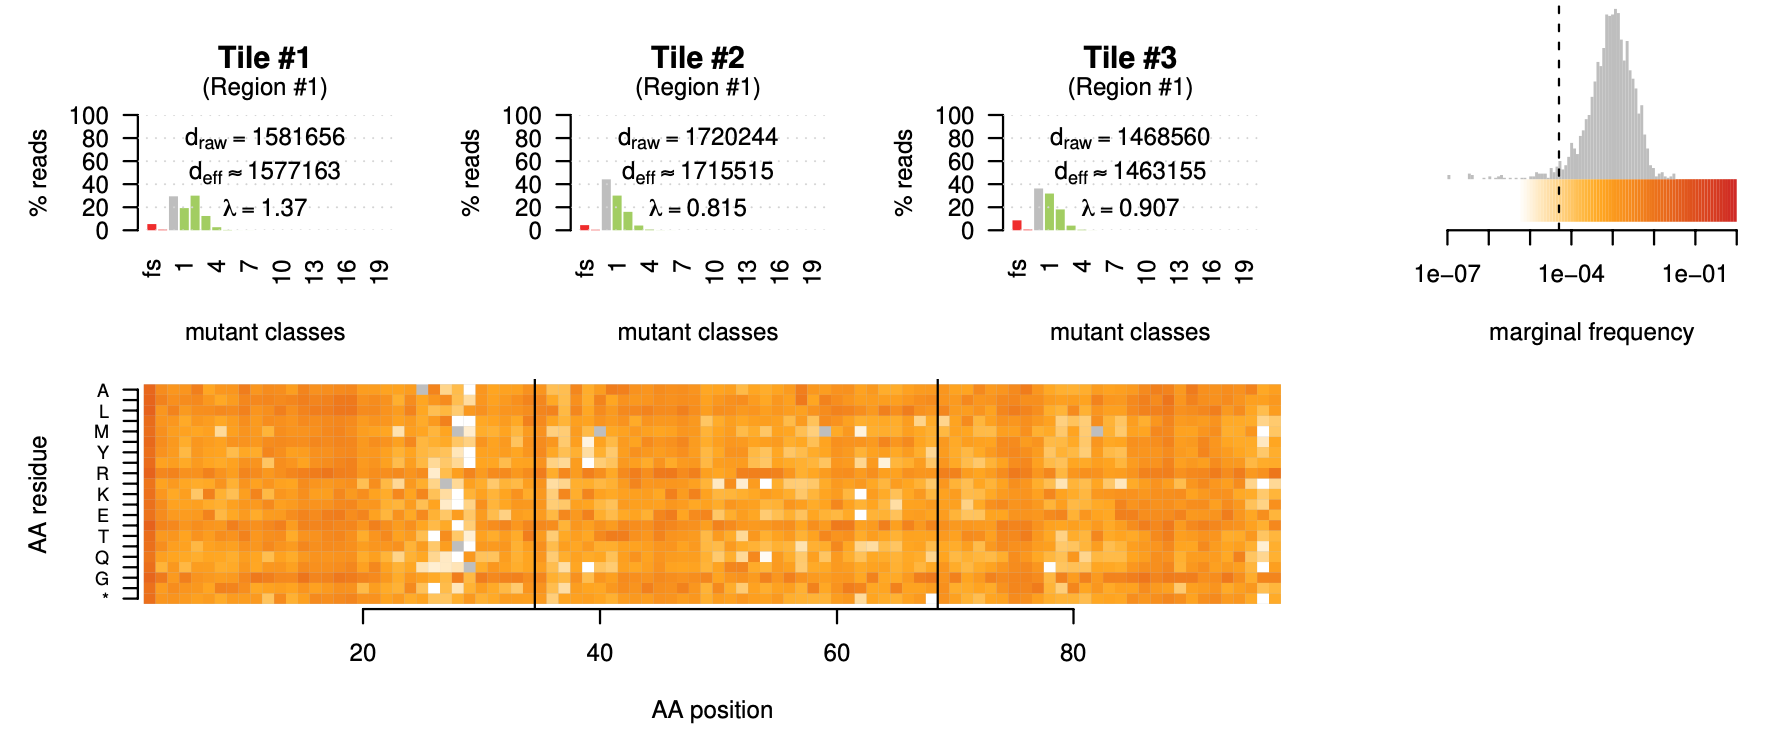
\includegraphics[width=.6\textwidth]{Figures/SUMO1/SUMO_coverage.png} }}%
%     \qquad
%     \subfloat[\centering Extrapolation for region 1]{{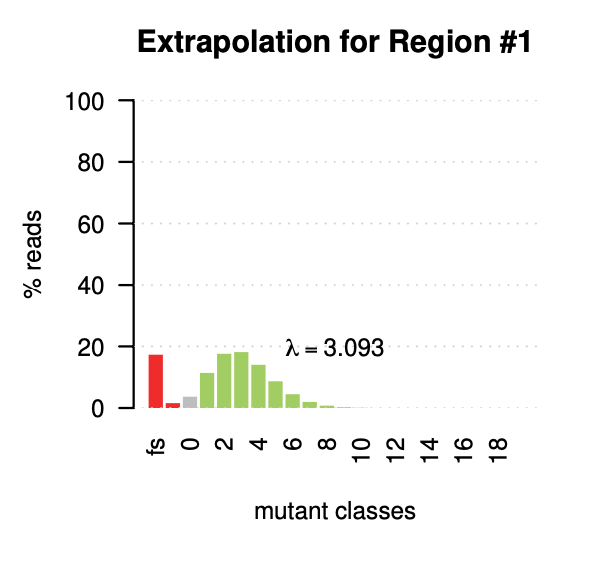
\includegraphics[width=.3\textwidth]{Figures/SUMO1/Extrapolation_R1.png} }}%
%     \caption{The coverage heatmap and an extrapolation of the number of variants per clone for Region 1 for the re-calculated SUMO1 map. The heatmap shows marginal frequencies for each amino acid change. $\lambda$ refers to the mean of the best fitting Poisson distribution of the number of variants observed per read.}%
%     \label{fig:heatmap}%
% \end{figure}


After filter application, there is a clear separation between the enrichment values of the nonsense and synonymous variants (Fig \ref{fig:BCE distribution}), indicating a reliable selection assay.
The missense variants enrichment values show a bimodal distribution, two modes are located at around -1.474 and  -0.3, which are slightly smaller than the nonsense and synonymous modes, which are around -1.212 and -0.025 respectively. In the case of the upper mode, this could indicate that most non-syononymous SUMO1 variants have at least a small fitness effect. For the lower mode however, it is unlikely that many variants are more deleterious than nonsense, so the shift may instead be an artifact of the harsher filtering approach.
% difference between the missense modes and nonsense/synonymous modes/
\begin{figure}[H]
    \centering
    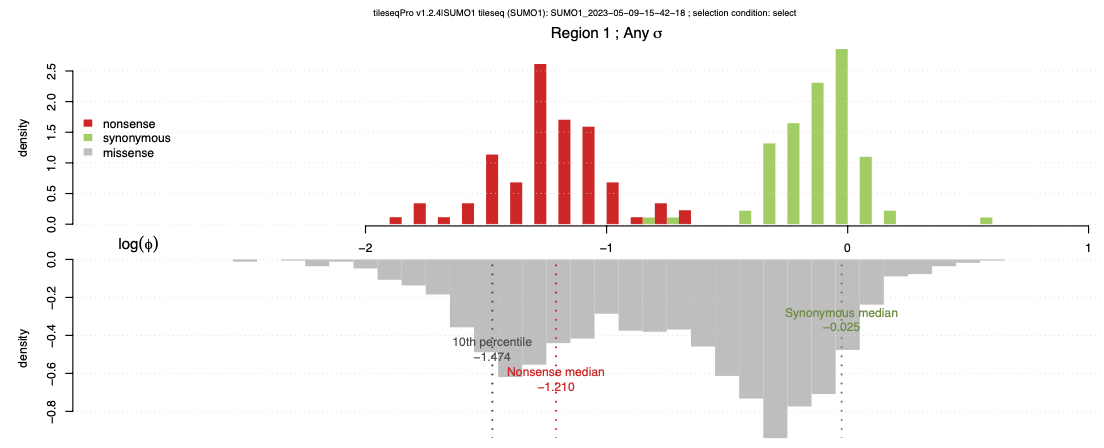
\includegraphics[width =.8\textwidth]{Figures/SUMO1/BCE.png}
    \caption{The enrichment ratio distributions of SUMO1 shows the overall distribution of missense(grey), synonymous(green), and nonsense(red) variants' enrichment values in region 1 of SUMO1 gene. }
    \label{fig:BCE distribution}
\end{figure}

\newpage


\subsubsection{Comparison between TileSeqPro and the Legacy pipeline}

A comparison of the maps created by TileSeqPro and the Legacy pipeline as visualized via Mavevis\cite{esposito_mavedb_2019} is shown in Figure \ref{fig:final map}. The first twenty amino acid are insensitive to missense mutaions in both version of variant effect maps as expected, since this region of SUMO1 is intrinsically disordered\cite{BAYER1998275}. The Legacy version of the map shows more available amino acid changes compared to our new version, especially near amino acid position 28, due to differences in filtering. 
%The possible reason for that is we filtered out codon changes that have low marginal frequencies before merging them into amino acid level scores in the updated pipelines; while in our old pipelines, we collapsed the equivalent codon changes and merged them into amino acid level change before filtering. Therefore, we have more available data generated from the old pipelines, at the expense of keeping low quality data points.

% final map 
\begin{figure}[H]%
    \centering
    \subfloat[\centering heatmap for SUMO1 2023 scores generated by Mavevis]{{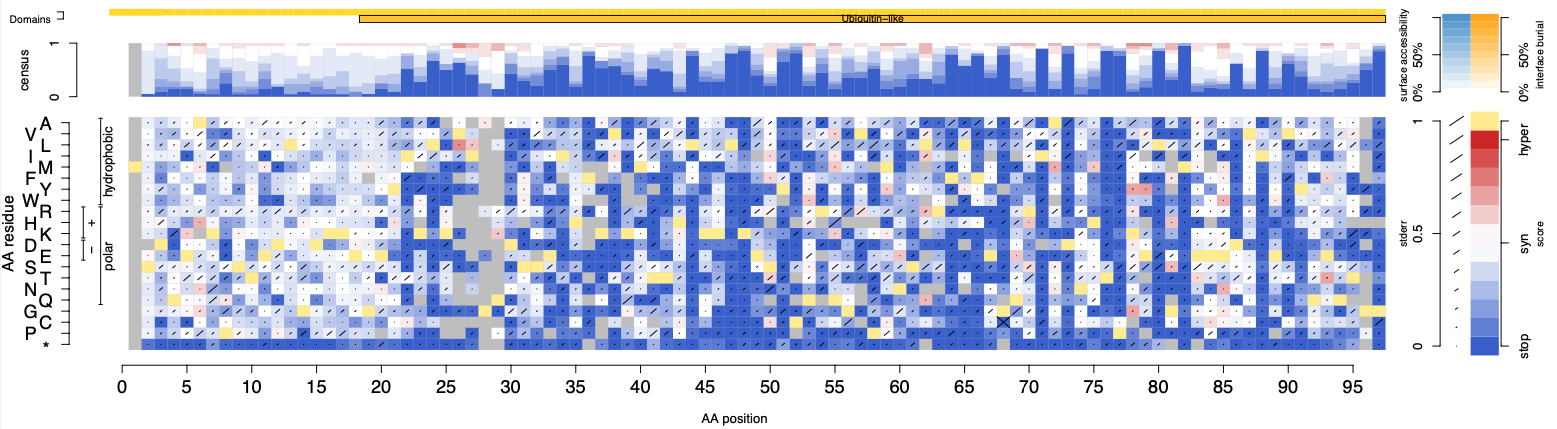
\includegraphics[width=.9\textwidth]{Figures/SUMO1/new_final_map.png} }}%
    \qquad
    \subfloat[\centering heatmap for SUMO1 2019 scores generated by Mavevis]{{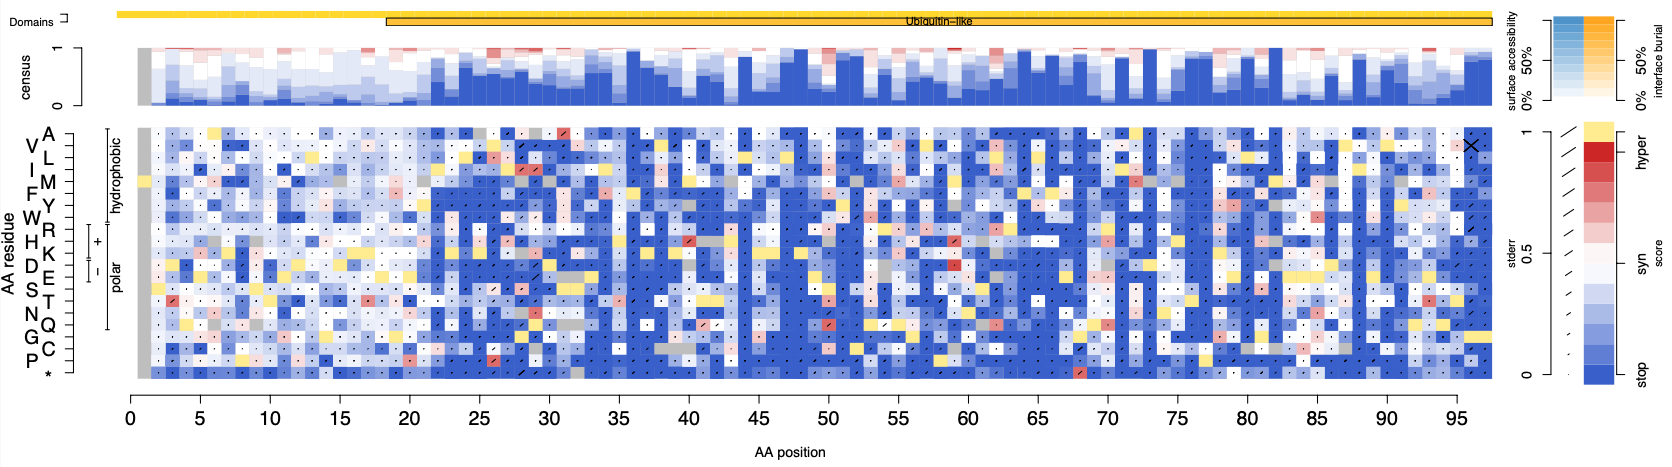
\includegraphics[width=.9\textwidth]{Figures/SUMO1/old_final_map.png} }}%
    \caption{A comparison of new and old version of SUMO1 heatmaps. The x-axis represents the amino acid position in protein, and the y-axis includes all possible amino acid changes. Colors used in the heatmap stand for the fitness score, where blue describes the variants which are as deleterious as full deletion; white represents synonymous-like variants, red stands for increased fitness than the wildtype residue at the given position; and yellow represents the wildtype amino acid.\cite{esposito_mavedb_2019}}%
    \label{fig:final map}%
\end{figure}



Missense and synonymous mutations, were assigned larger estimates of standard error by TileseqPro compared to Legacy (see supplemental Fig. 3). The reason for this change might be due to the introduction of bootstrapping and more pessimistic error regularization methods.

% \begin{figure}[H]
%     \centering
%     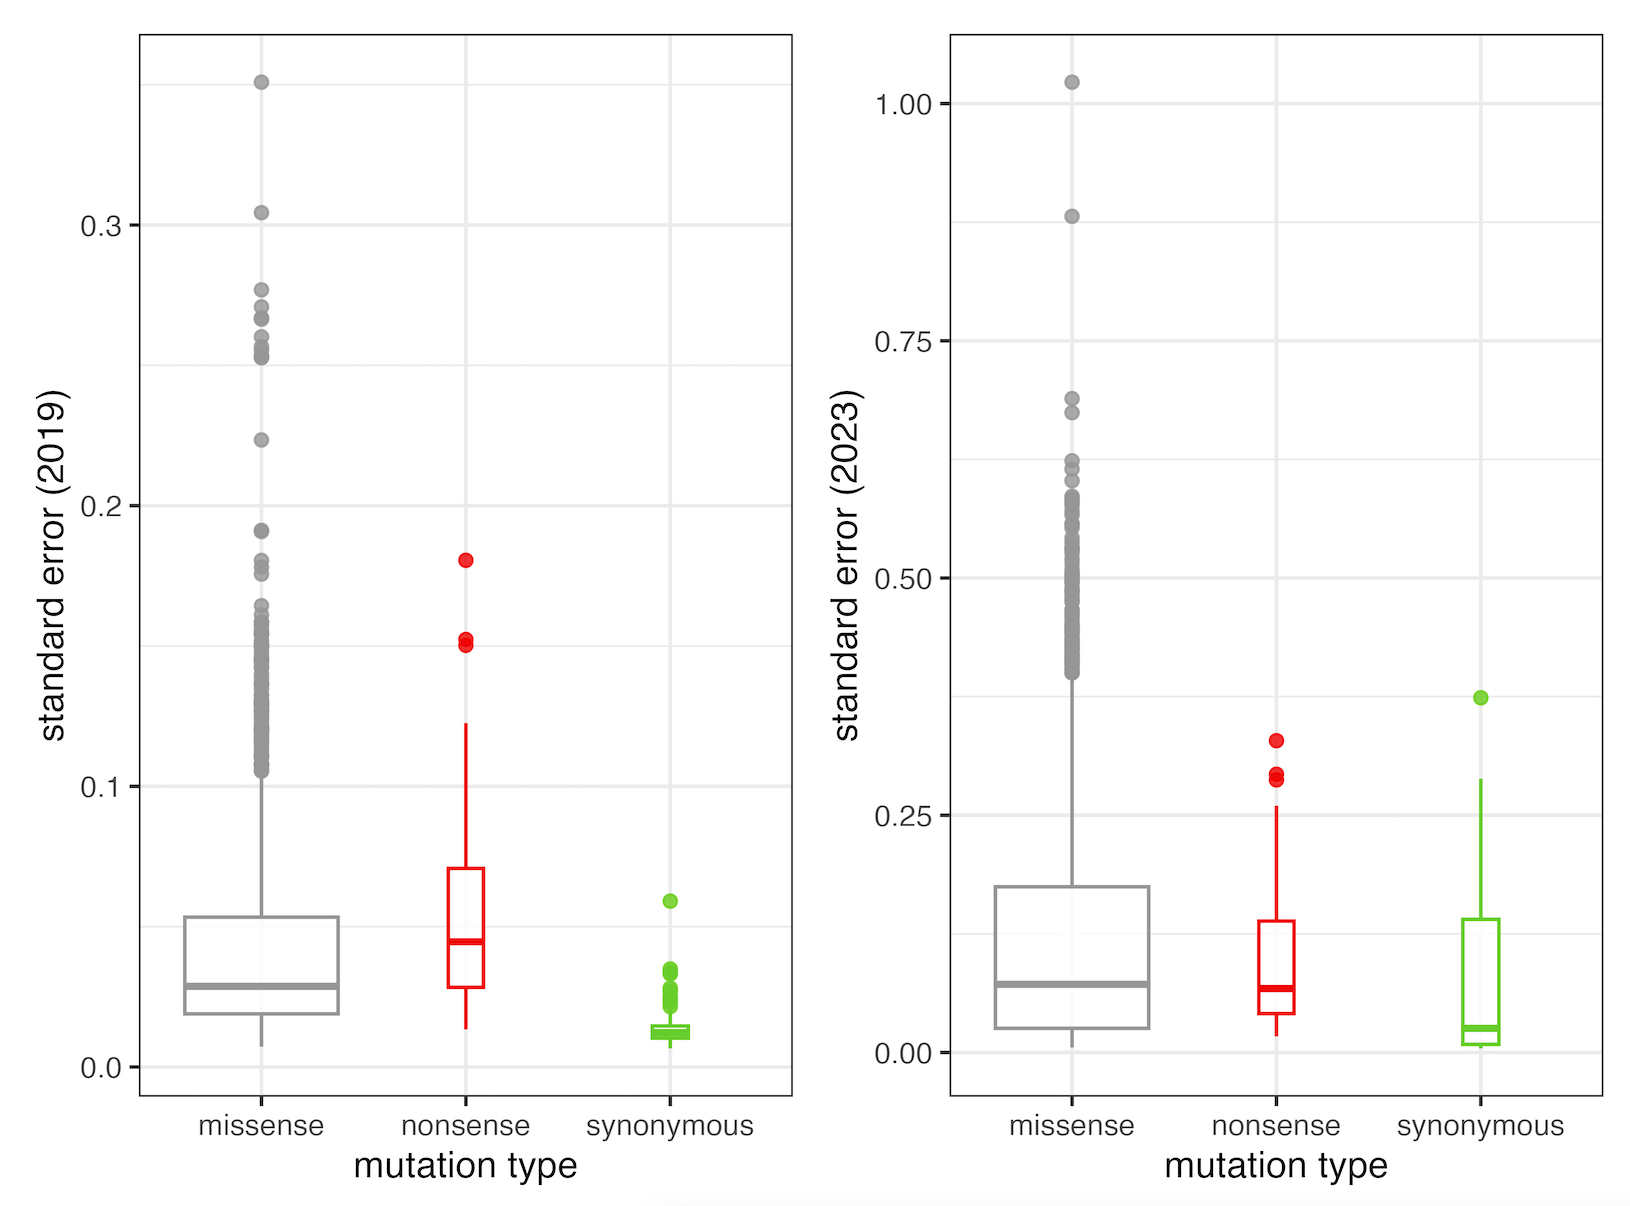
\includegraphics[width =.4\textwidth]{Figures/SUMO1/standard_error.png}
%     \caption{The distribution of standard error of new and old fitness scores.}
%     \label{fig:se boxplot}
% \end{figure}

Overall, the correlation between the fitness scores produced by the two  pipelines is high with Spearman's $\rho = 0.95$ (see supplemental Fig. 4). Interestingly, a moving window analysis of the correlation also indicates slightly less agreement between two in the N-terminal disordered region.


% * Discussion of why there is no good reference set for SUMO1 (not a disease gene) and that PRC and LLR analysis were skipped accordingly.
\subsubsection{Moving Window Correlation between Fitness Scores and VARITY Scores}
Since SUMO1 is not a disease gene, no reference set for precision-recall analysis in terms of pathogenicity exists. As an alternative evaluation approach, we analysed the correlation of fitness scores with the computational predictor VARITY\cite{wu_improved_2021}.  As expected, there is substantial anti-correlation between the VARITY probability of pathogenicity and fitness scores (they are scaled oppositely). Disregarding the disordered region (the first 20 amino acids), from position 25 to 70, the Legacy fitness scores are more anti-correlated with VARITY\_R and VARITY\_ER scores; whereas from position 70 to the end, the new fitness scores have better anti-correlation (Fig. \ref{fig:VARITY_SUMO}). The overall value of $\rho$ in these regions fluctuates around approximately $-0.5$.

\begin{figure}[H]%
    \centering
    \subfloat[\centering Correlation between VARITY\_R Scores and Fitness Scores]{{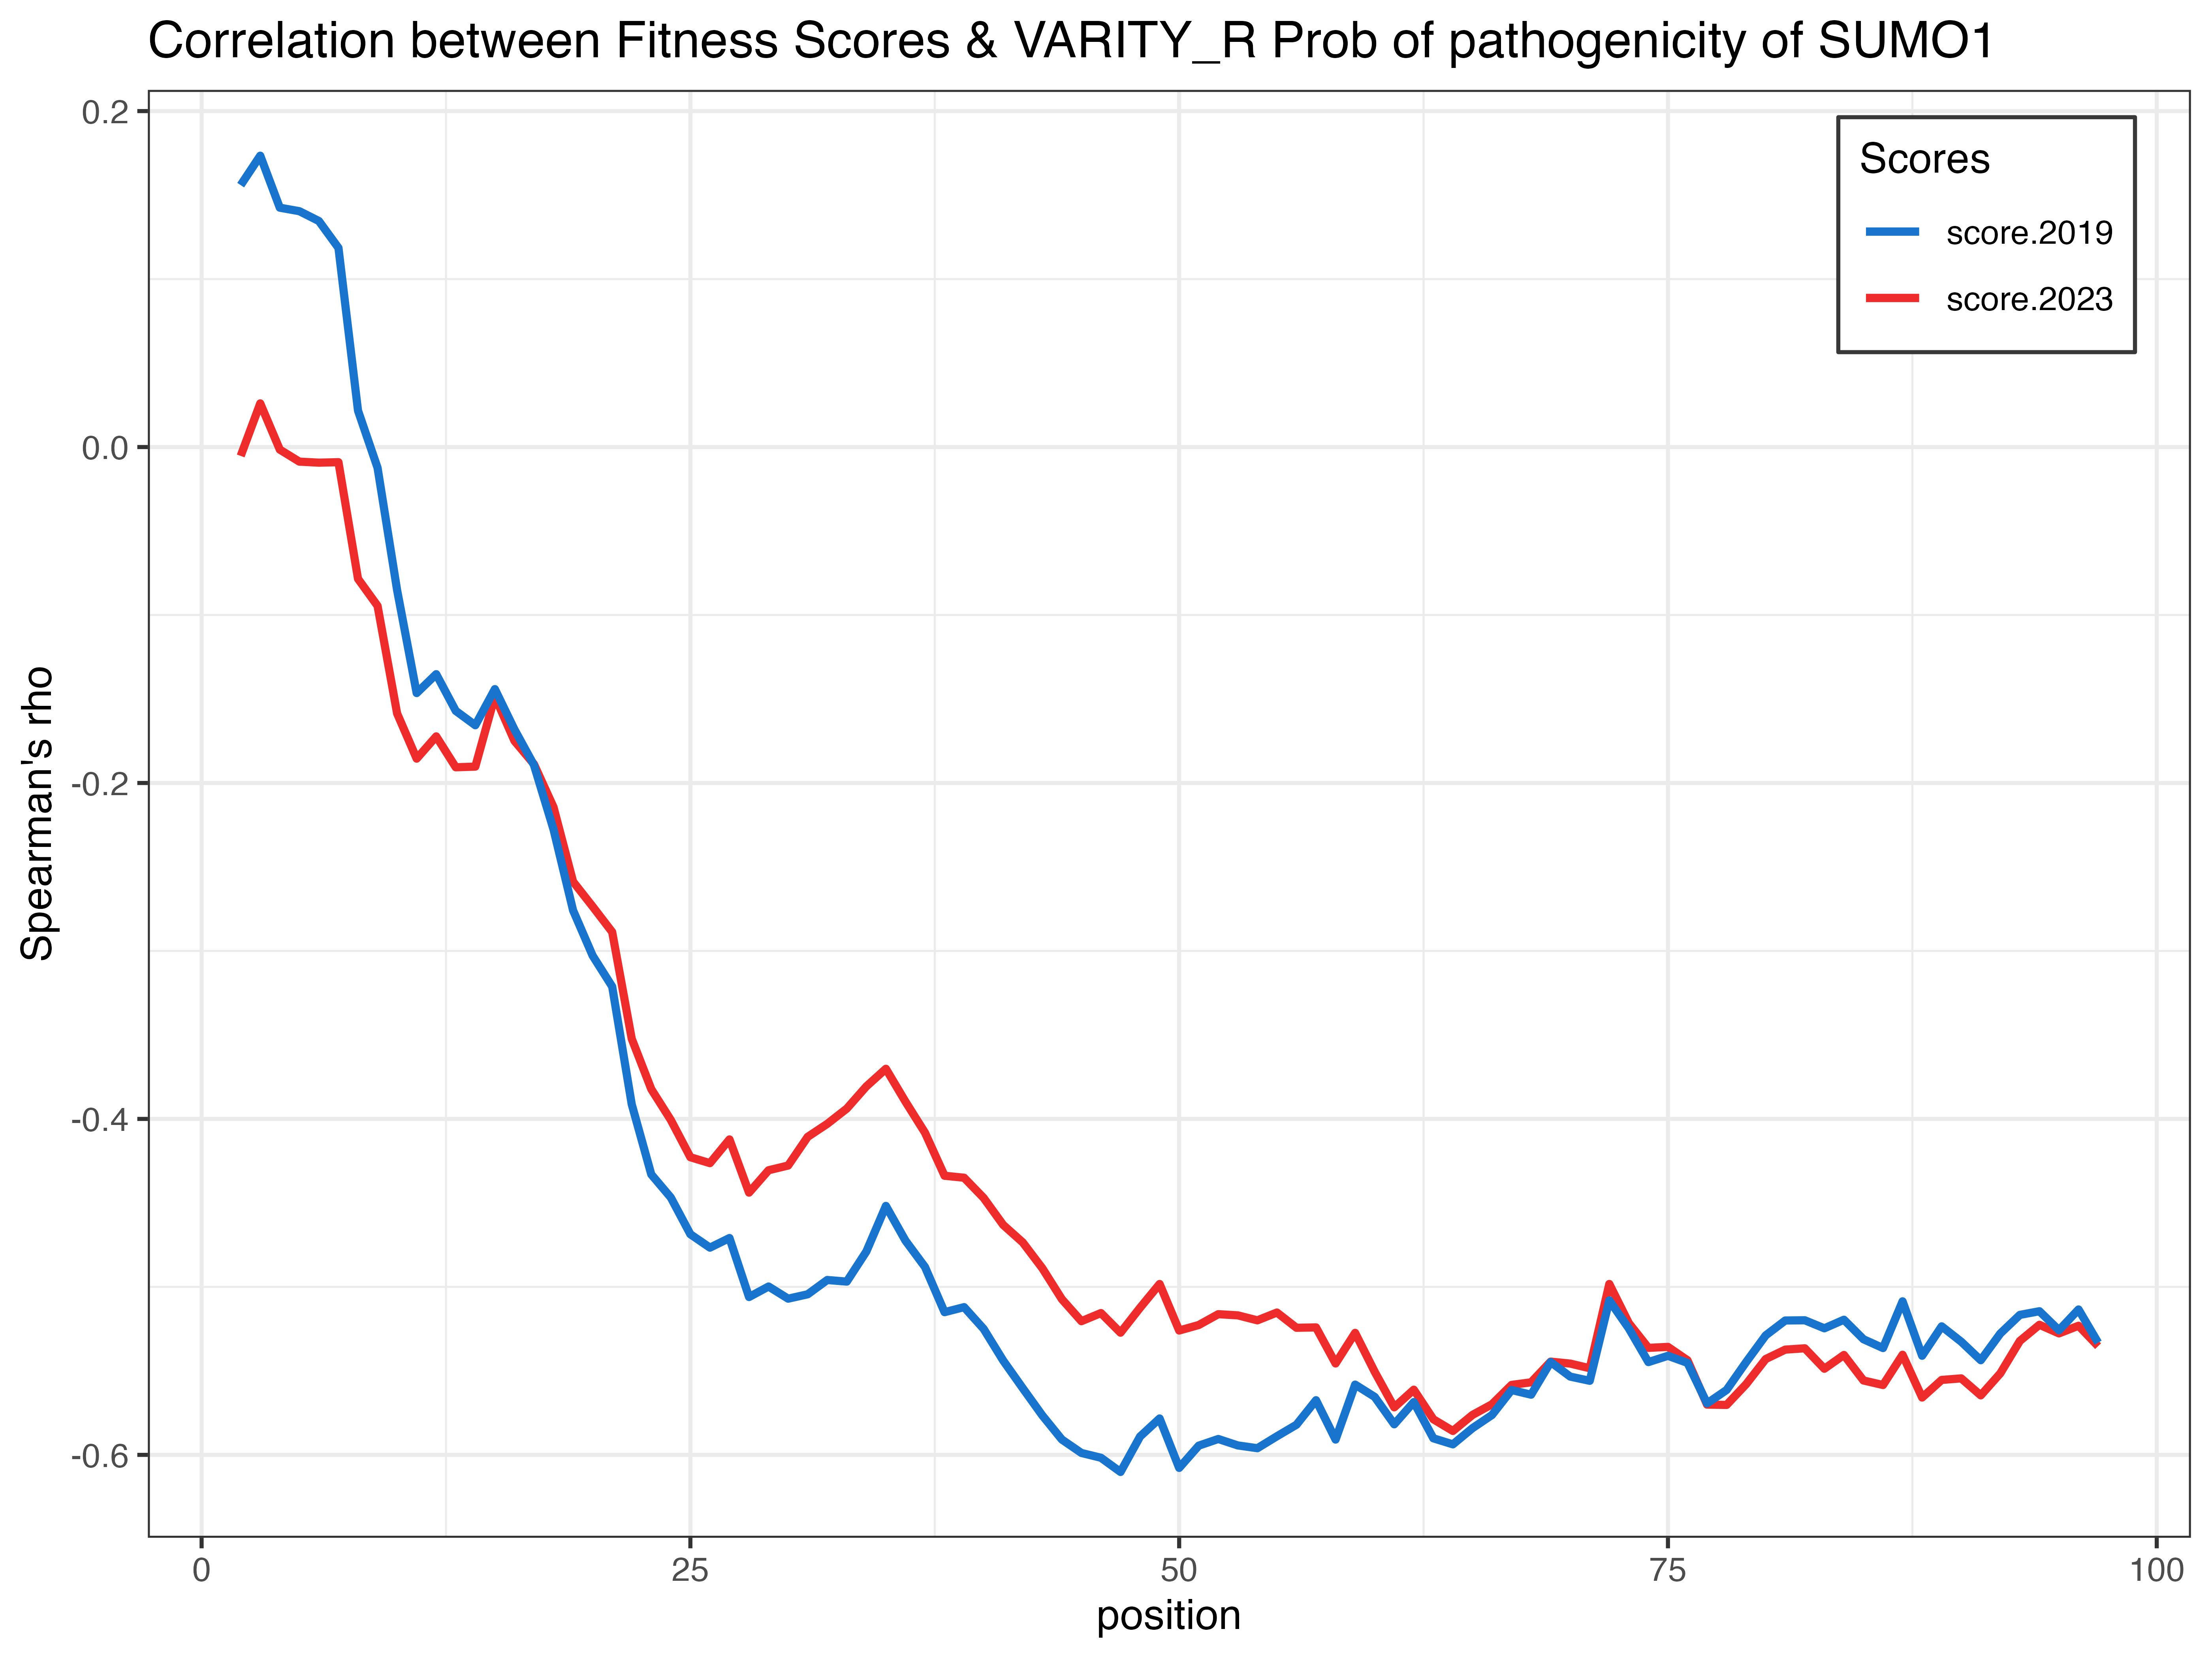
\includegraphics[width=.45\textwidth]{Figures/SUMO1/spearman_VARITY_R.png} }}%
    \qquad
    \subfloat[\centering Correlation between VARITY\_ER Scores and Fitness Scores]{{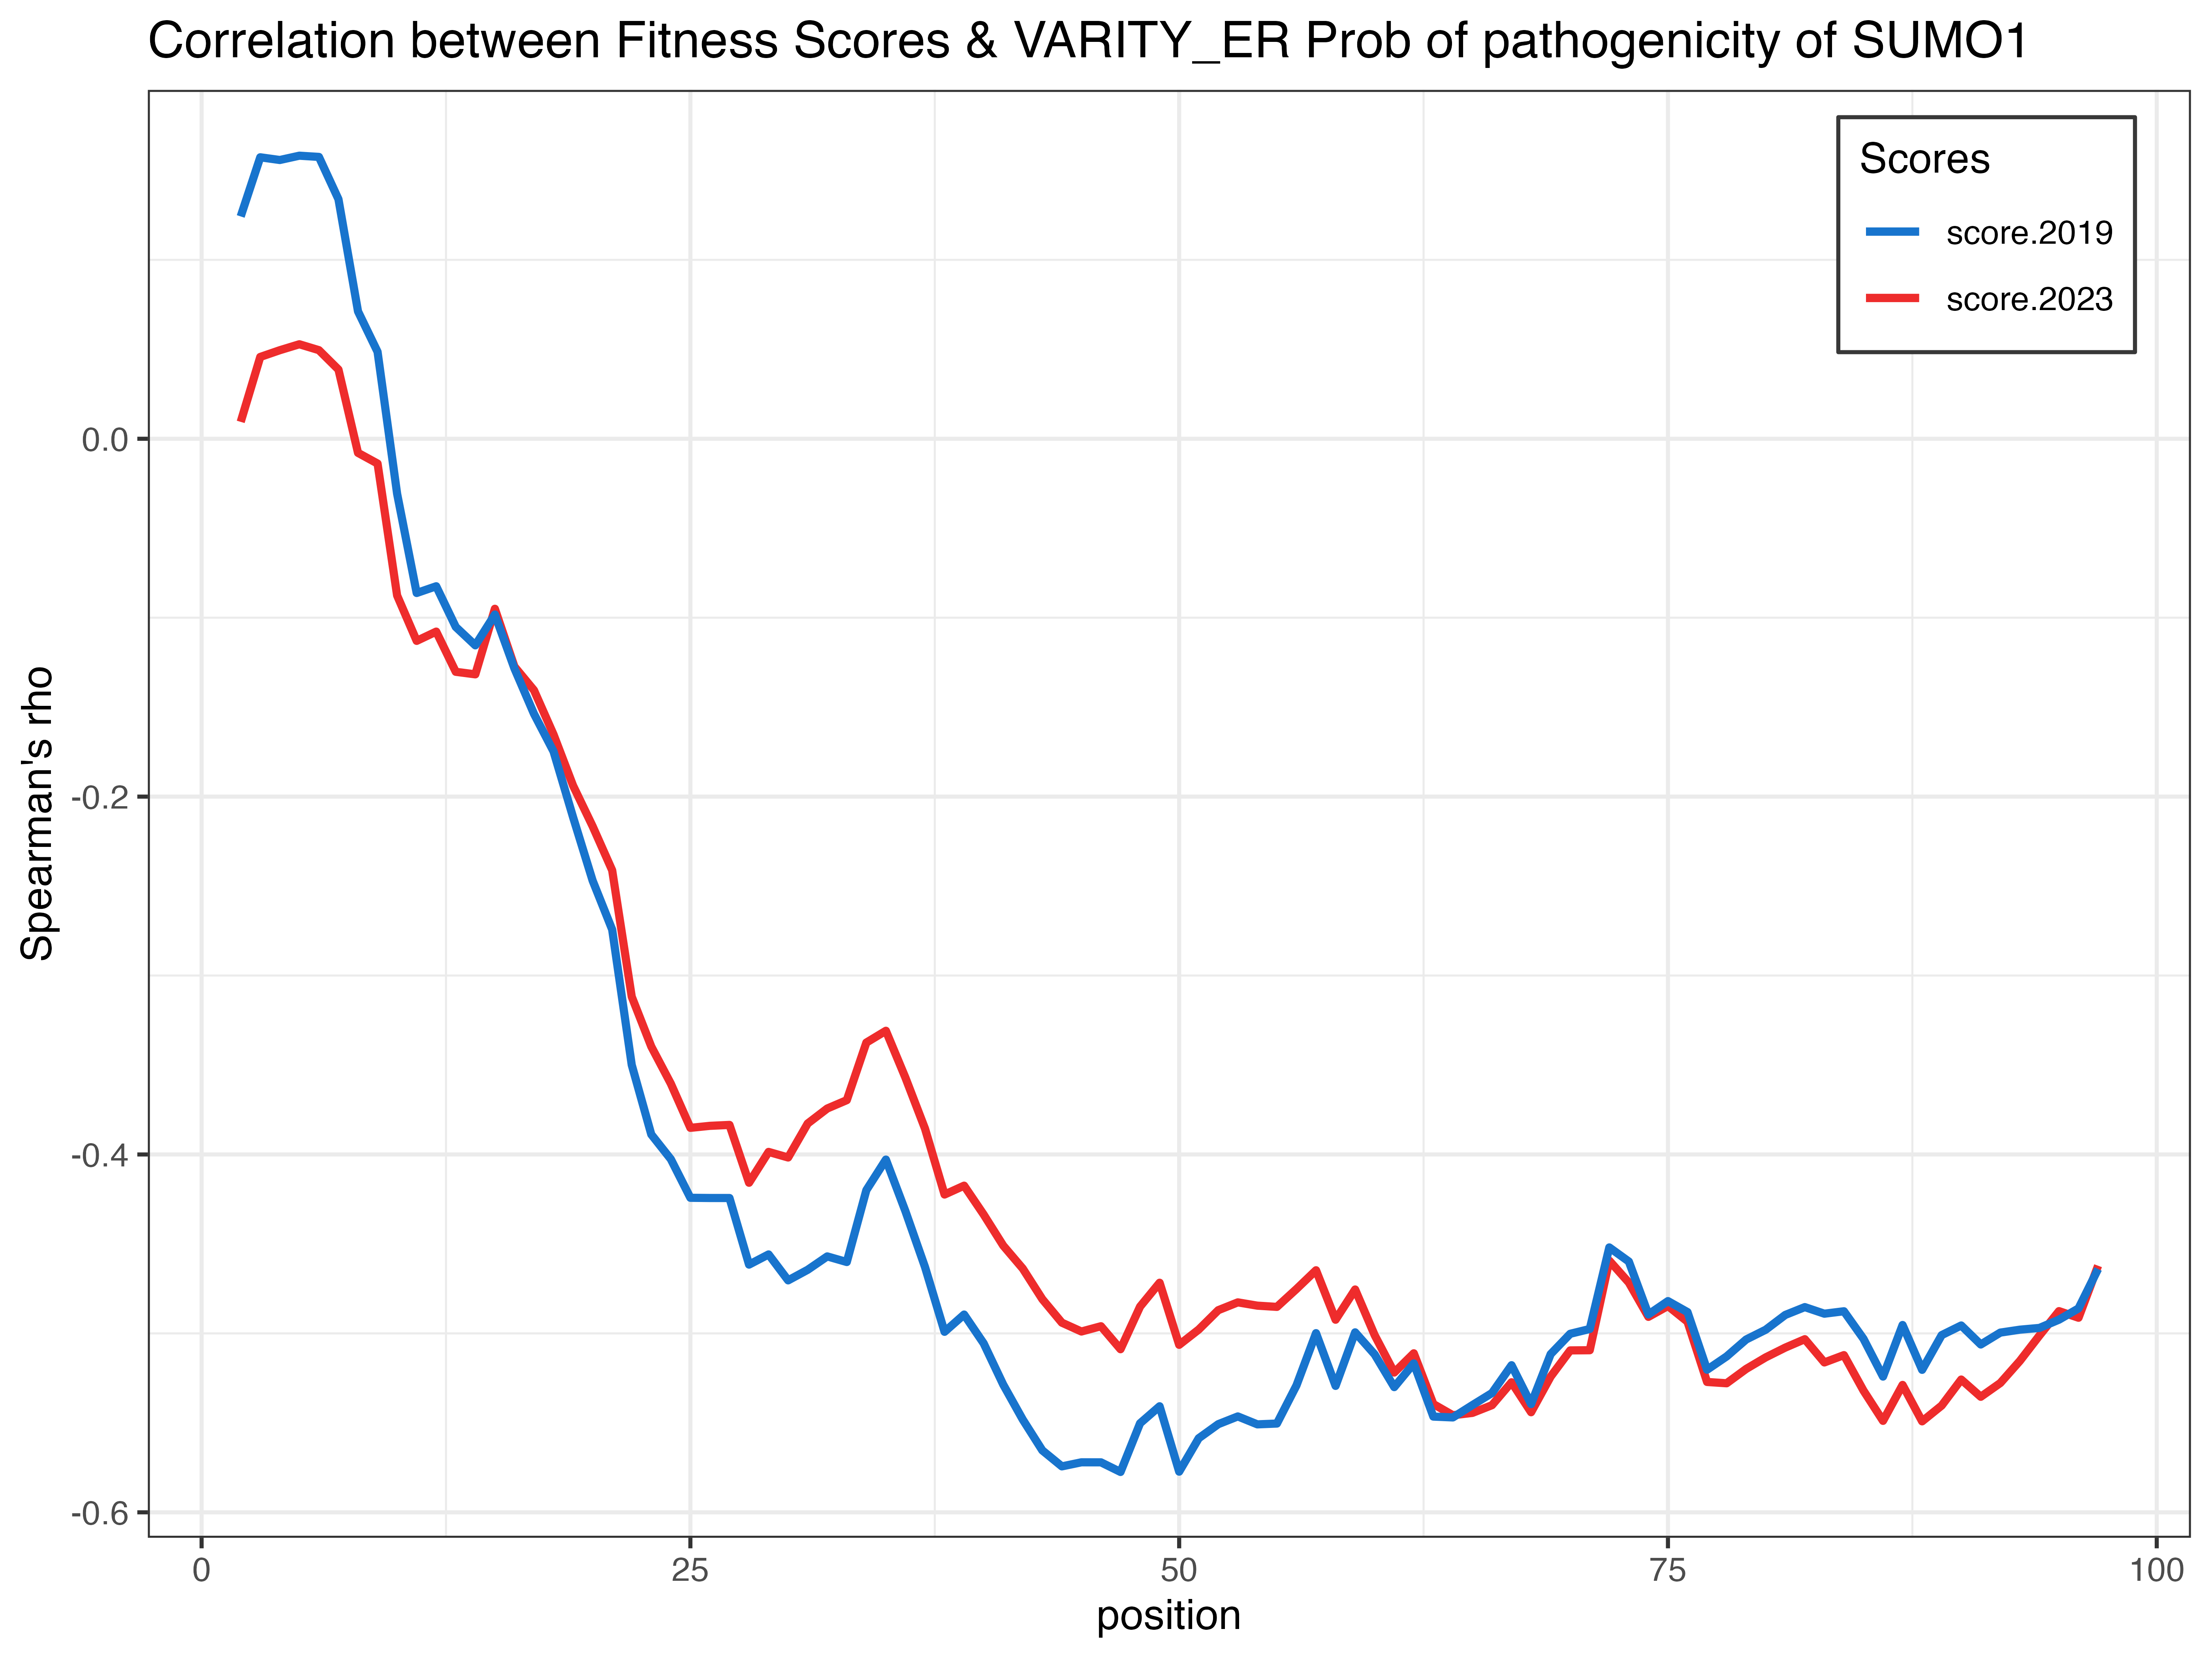
\includegraphics[width=.45\textwidth]{Figures/SUMO1/spearman_VARITY_ER.png} }}%
    \caption{Moving window correlation between VARITY Scores and Fitness Scores. Blue line represents the old scores, while red line represents the updated scores.}%
    \label{fig:VARITY_SUMO}%
\end{figure}
% * ==> Which map performed better?
\subsubsection{Conclusion}
Both version of SUMO1 maps performed similarly in terms of correlation between VARITY scores. Our updated TileseqPro pipelines used more information on generating the error estimates, whereas the harsher filtering steps in the TileseqPro pipelines caused measurement error we revealed in the variant enrichment value distribution. Additionally, amino acid changes with low marginal frequencies were filtered out in the updated map while they presented in the previous version of SUMO1 map.


\subsection{CALM1}
We then re-processed the map for CALM1, which was first created by the Roth Lab in 2018 and first updated by 2019\cite{floyd_proactive_2023}.
\subsubsection{Observations from QC results}

% coverage
The library shows an extrapolated average number of 2 amino acid changes per clone (see supplemental Fig. 5). The overall coverage appears low, with many low-frequency variants (white in the figure) or outright missing ones (gray in the figure).

% \begin{figure}[H]%
%     \centering
%     \subfloat[\centering coverage heatmap]{{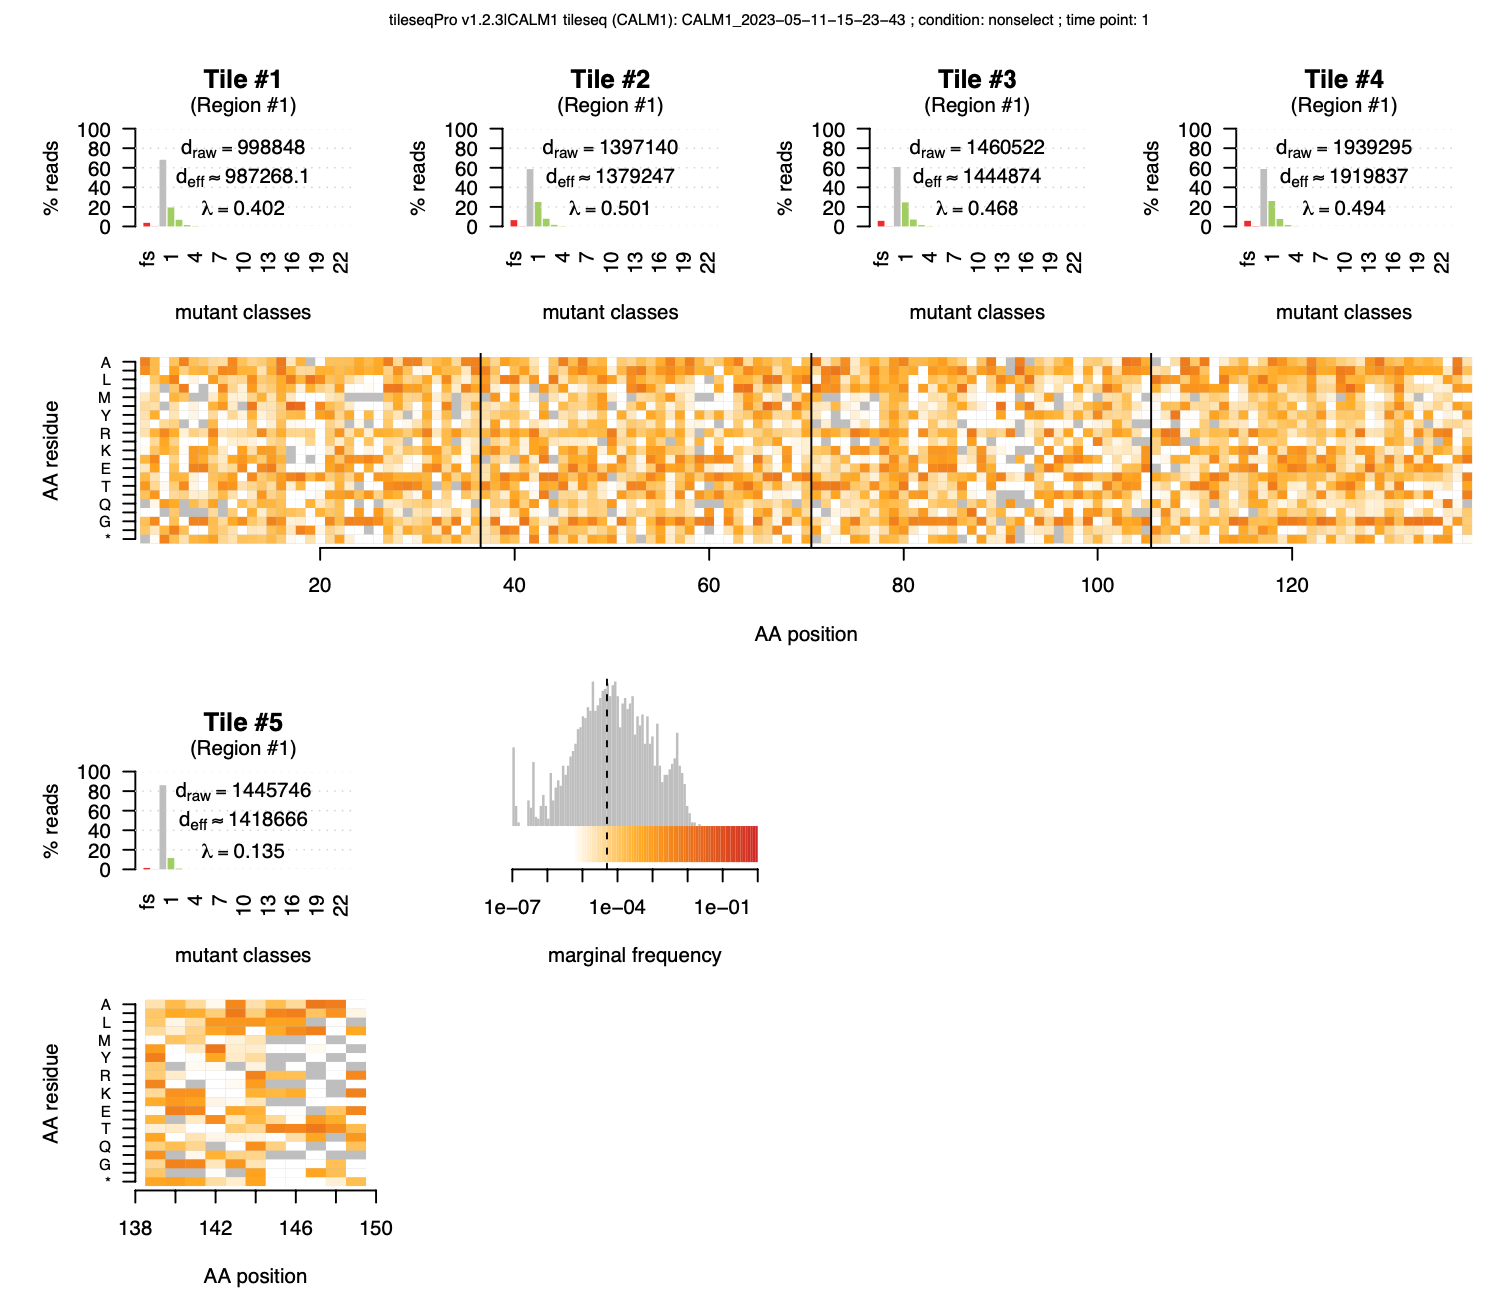
\includegraphics[width=.6\textwidth]{Figures/CALM1/coverage.png} }}%
%     \qquad
%     \subfloat[\centering Extrapolation for region 1]{{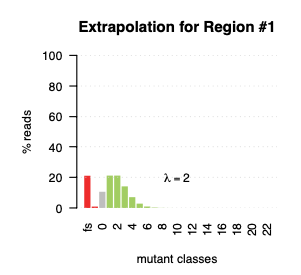
\includegraphics[width=.3\textwidth]{Figures/CALM1/extrapolation_CALM1.png} }}%
%     \caption{The coverage heatmap and an extrapolation of the number of variants per clone for Region 1 for the re-calculated CALM1 map. The heatmap shows marginal frequencies for each amino acid change. Lambda refers to the mean of the best fitting Poisson distribution of the number of variants observed per read.}%a
%     \label{fig:heatmap_CALM1}%
% \end{figure}


% filtering
Examining the distribution of synonymous and nonsense variant enrichment ratios ($\log(\phi)$) relative to marginal frequency (see supplemental Fig. 6 (a)) reveals that separation between $\log(\phi)$ improves noticeably at a frequency of $10^{-3.85}$. Given the sequencing depth of 1.4M reads per sample, we chose a minimum read count threshold of 200. After setting filters accordingly, around two third of variants were filtered out by frequency filter and bottleneck filters (see supplemental Fig. 6 (b)). 

% \begin{figure}[H]%
%     \centering
%     \subfloat[\centering $\log(\phi)$ bias plot]{{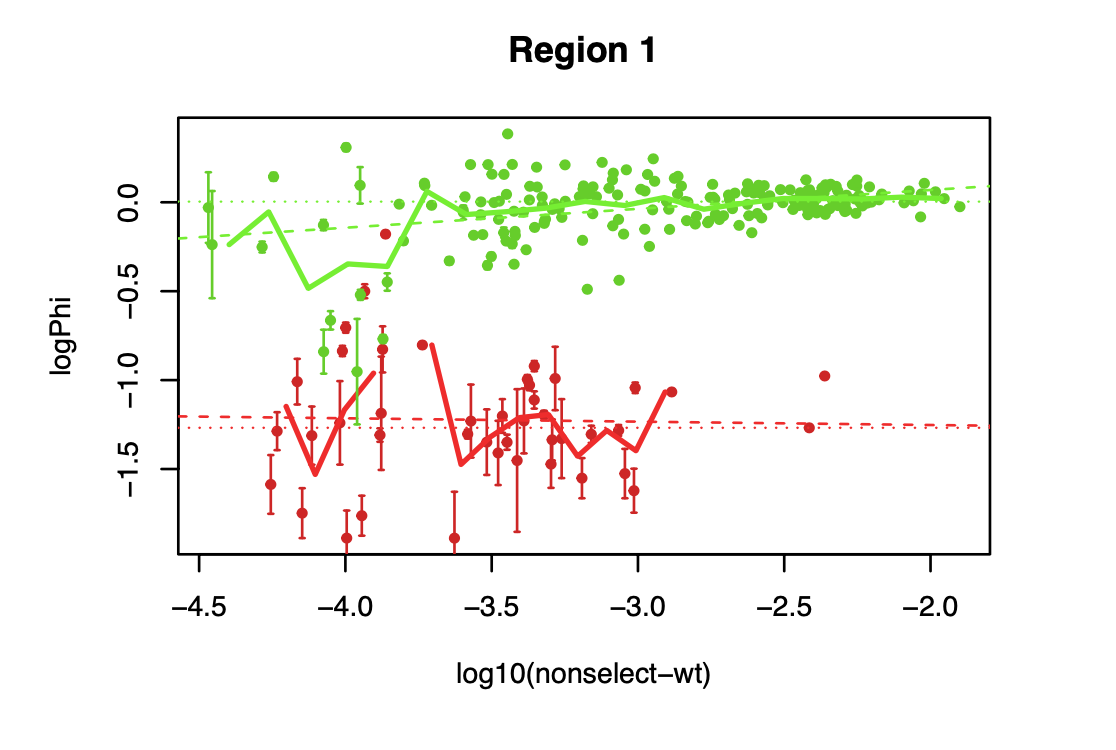
\includegraphics[width=.45\textwidth]{Figures/CALM1/logphi_bias.png} }}%
%     \qquad
%     \subfloat[\centering filtering breakdown]{{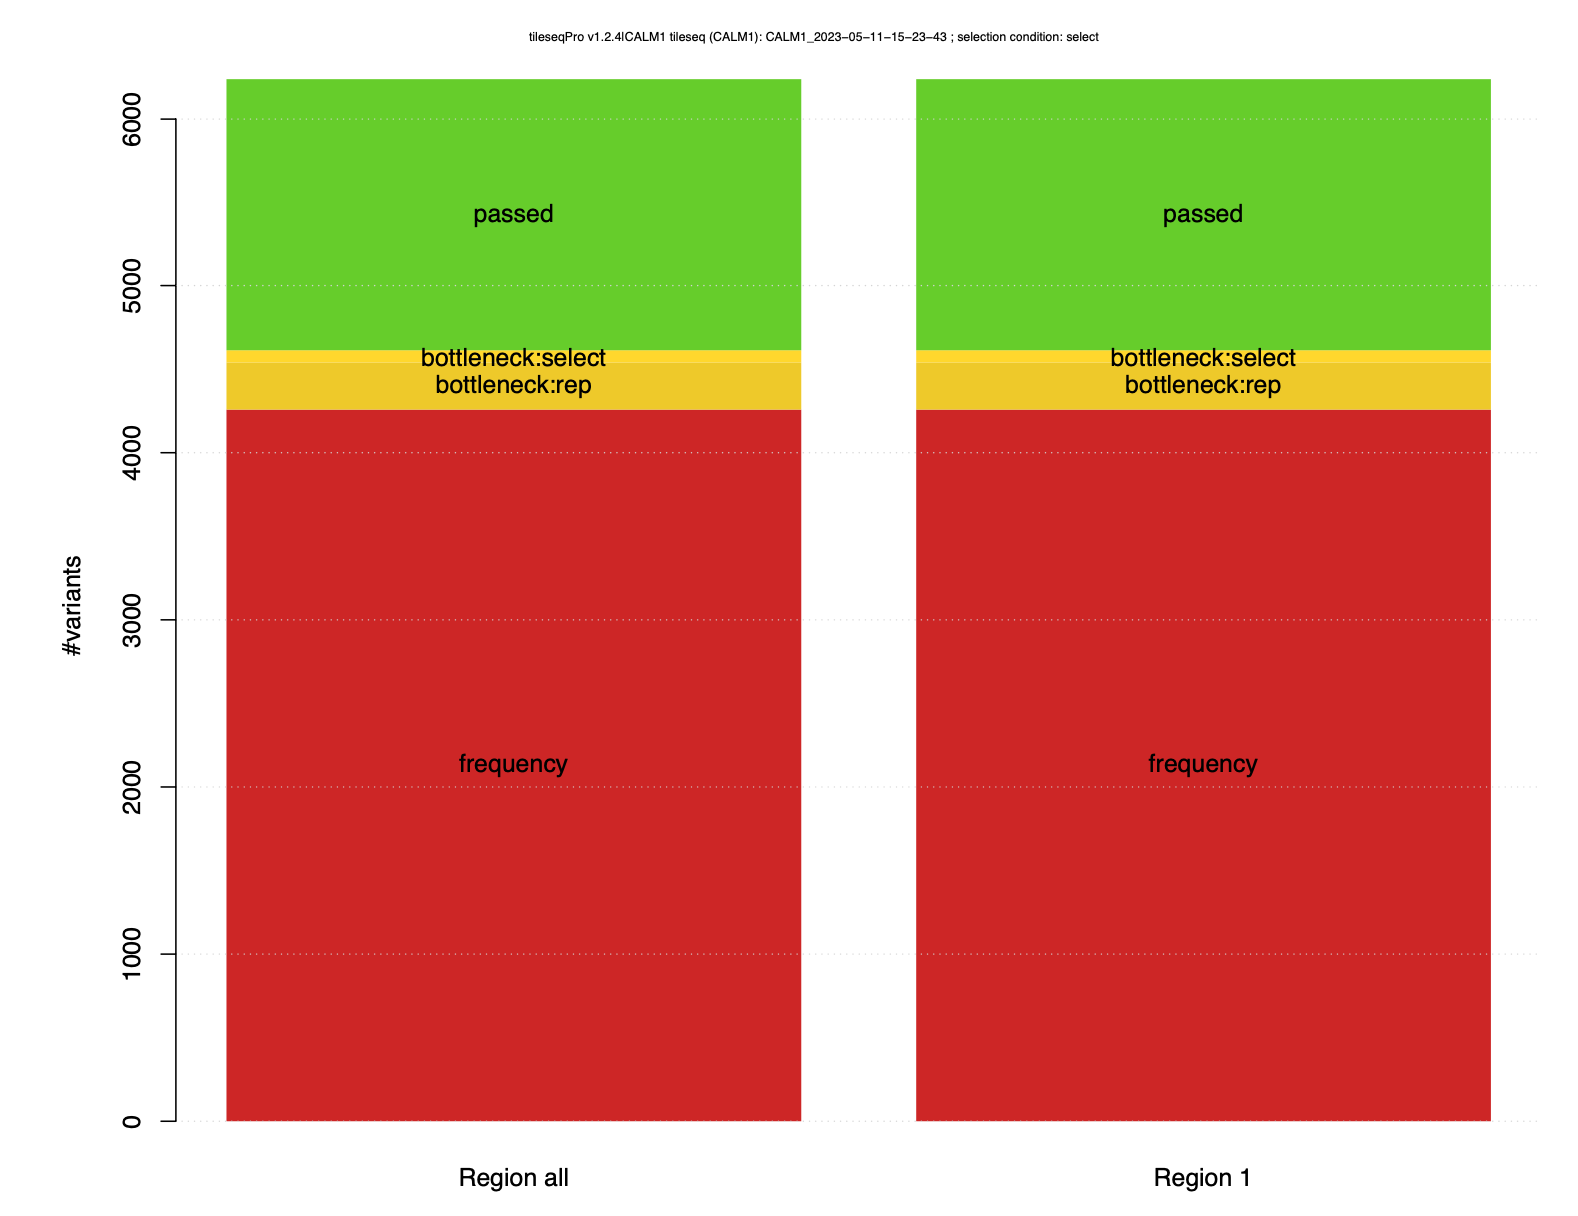
\includegraphics[width=.45\textwidth]{Figures/CALM1/filtering.png} }}%
%     \caption{The $log(\phi)$ bias plot and the filtering breakdown bar plot for CALM1 map. The $log(\phi)$ bias plot illustrates how the $\log(\phi)$ values of synonymous(green) and nonsense(red) variants changing as the read frequency cutoff increasing. The filtering breakdown plot show the number of CALM1 variants in region 1 that were subjected to individual filters.}%
%     \label{fig:filtering_CALM1}%
% \end{figure}

% logphi didtribution

Following these filter settings, there is a clear separation between the enrichment values of the nonsense and synonymous variants (Fig. \ref{fig:BCE distribution CALM1}), with modes located at -1.230 and 0.001 respectively, whereas the missense variants have only one mode near 0.001 with an extended shoulder towards the low end. This agrees with previous observations that most missense variants of CALM1 are not very damaging in terms of fitness\cite{weile_framework_2017}.


\begin{figure}[H]
    \centering
    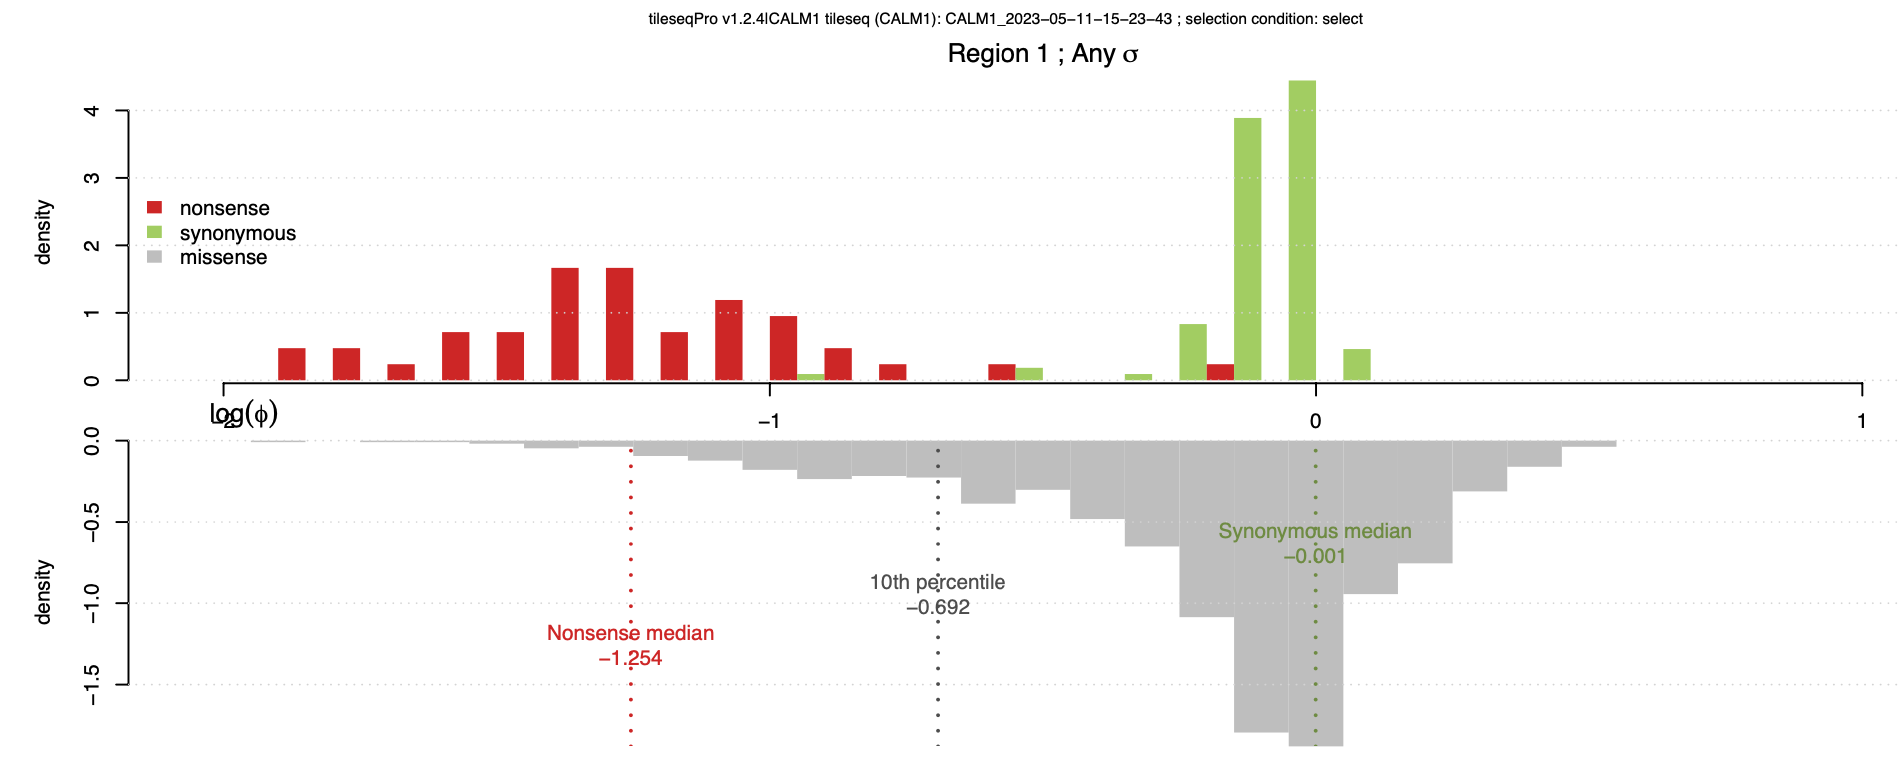
\includegraphics[width =.7\textwidth]{Figures/CALM1/BCE.png}
    \caption{The enrichment ratio distributions of CALM1 shows the overall distribution of missense(grey), synonymous(green), and nonsense(red) variants' enrichment values in region 1 of CALM1 gene. }
    \label{fig:BCE distribution CALM1}
\end{figure}

% mavevis heatmap
A comparison between the maps calculated via TileSeqPro and the Legacy pipeline is shown in Figure \ref{fig:final map CALM1}. The impact of harsh filtering in the new map is clearly visible, as almost 2/3 of variants were removed. This updated version CALM1 map could be a perfect candidate for machine learning imputation.

\begin{figure}[H]%
    \centering
    \subfloat[\centering heatmap for CALM1 2023 scores generated by Mavevis]{{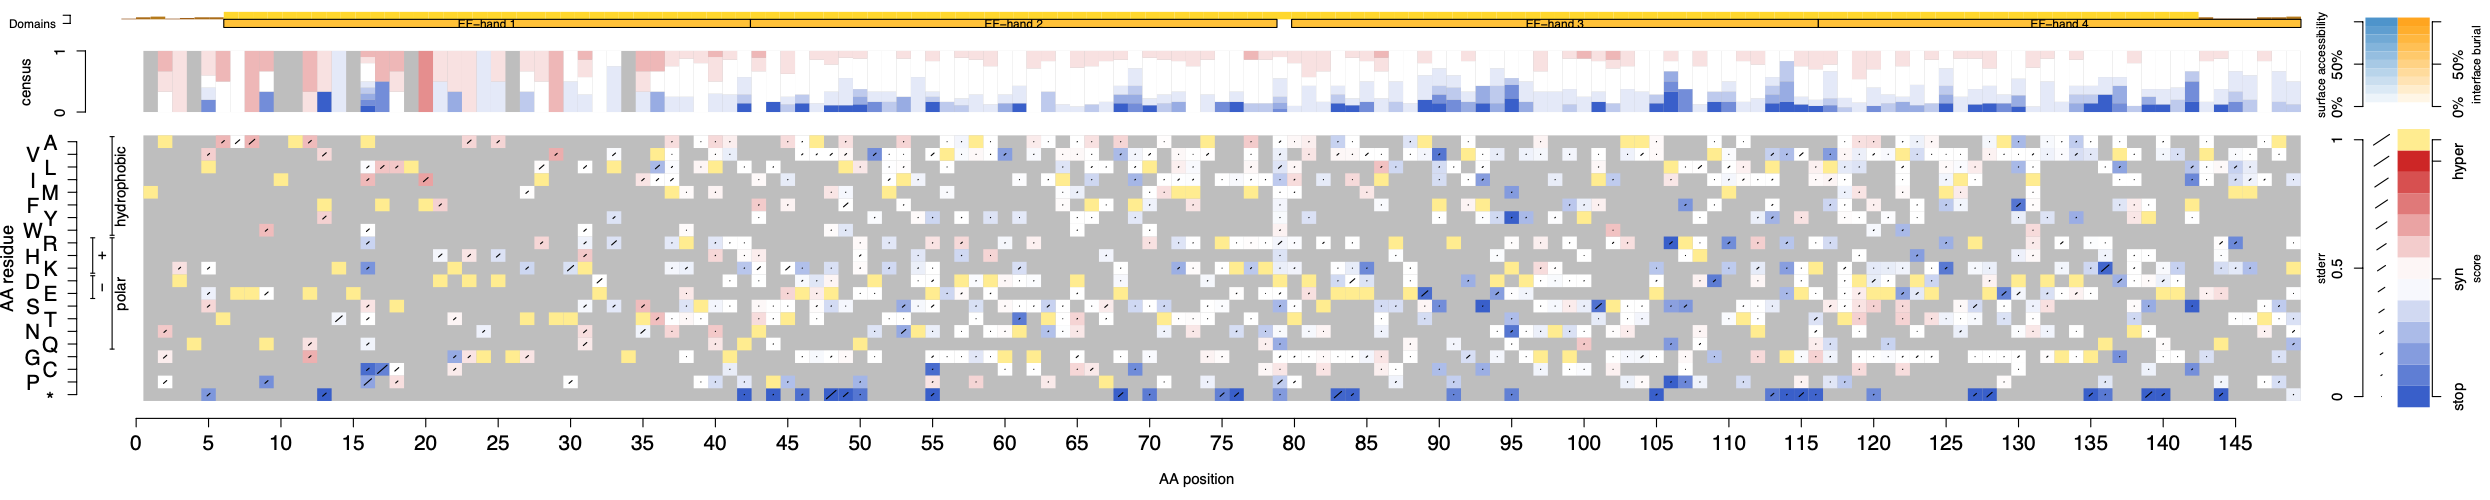
\includegraphics[width=.9\textwidth]{Figures/CALM1/new_heatmap.png} }}%
    \qquad
    \subfloat[\centering heatmap for CALM1 2019 scores generated by Mavevis]{{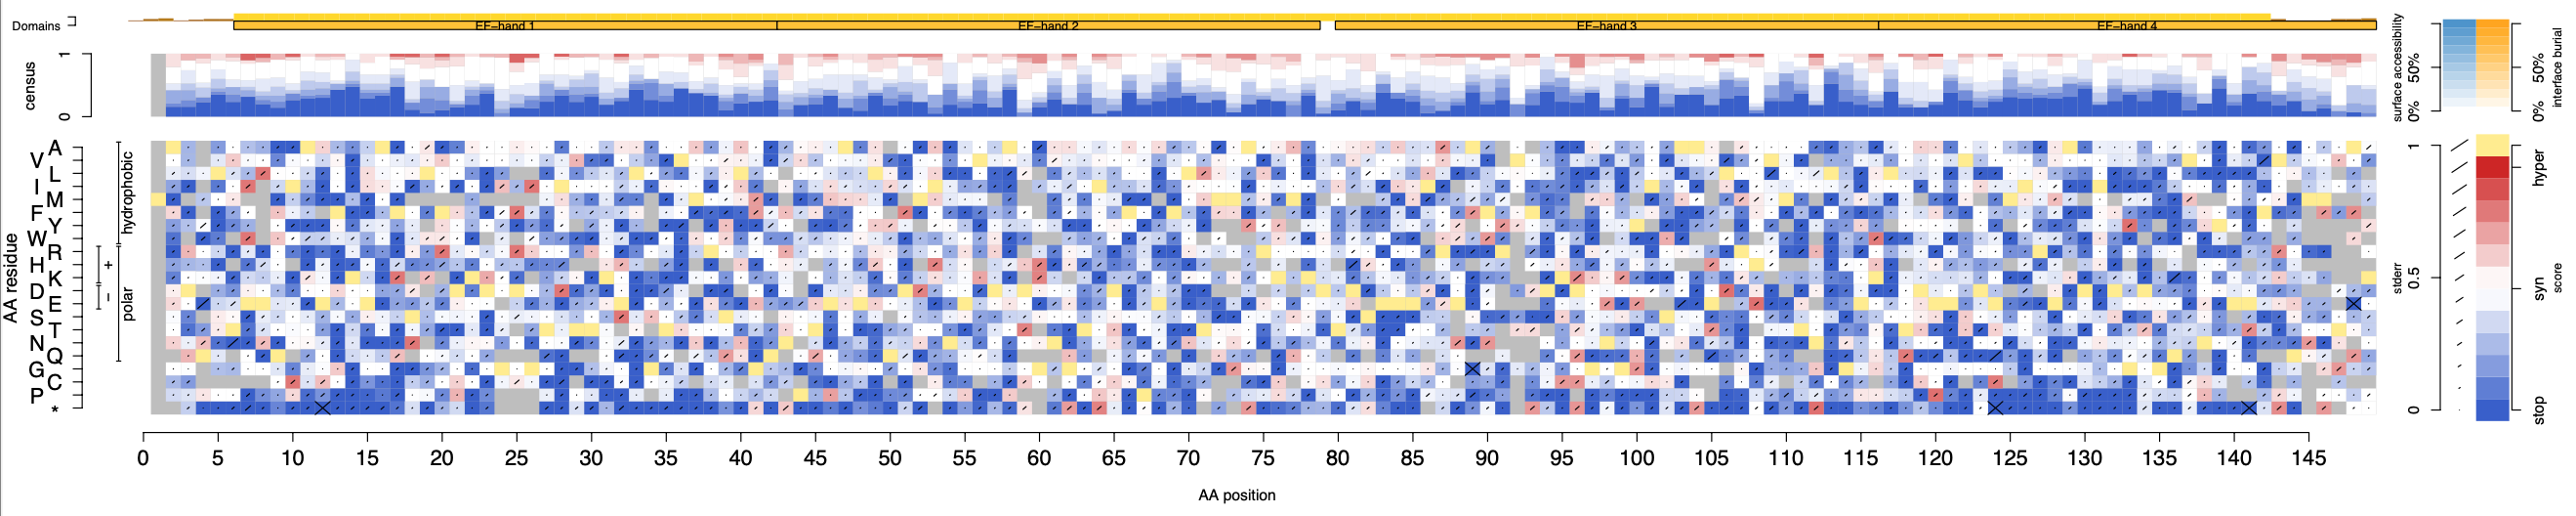
\includegraphics[width=.9\textwidth]{Figures/CALM1/old_heatmap.png} }}%
    \caption{A comparison of new and old version of CALM1 heatmaps generated by Mavevis.}%
    \label{fig:final map CALM1}%
\end{figure}

\subsubsection{Precision-recall Curve and Log-likelihood Ratio of Pathogenicity}
% PRC
\begin{figure}[H]
    \centering
    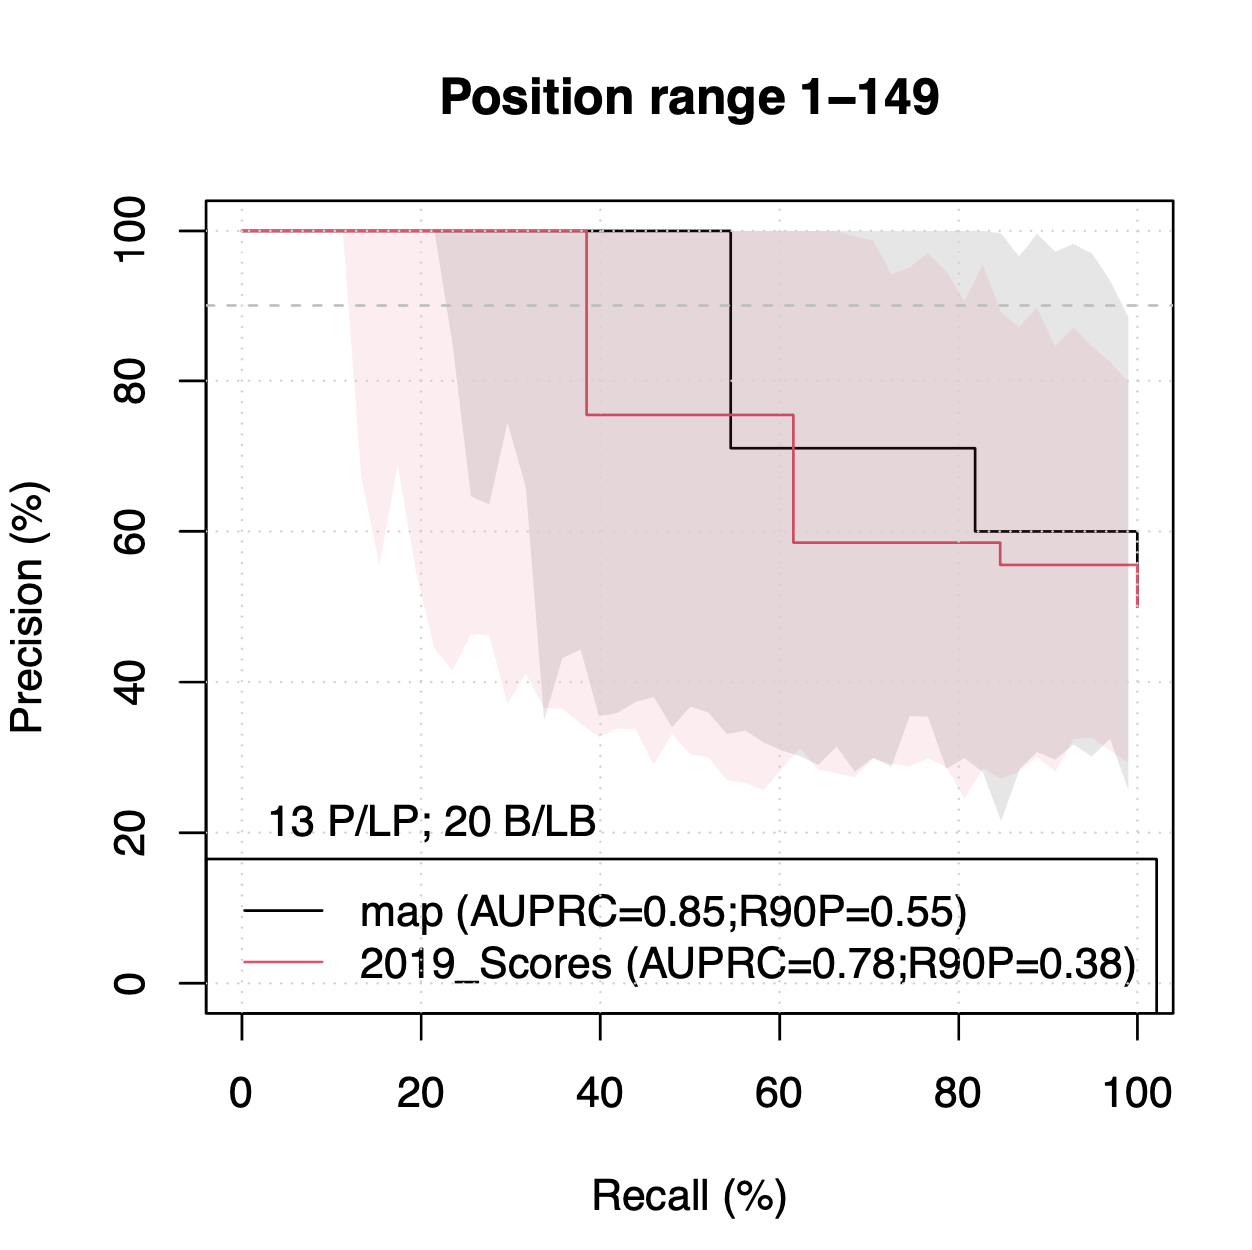
\includegraphics[width =.4\textwidth]{Figures/CALM1/update_PRC.png}
    \caption{Precision-recall Curve for the 2023 and 2019 version of CALM1 maps. The black line represents the curve for 2023 map, and the red line represents the curve for 2019 map. Reference sets this PRC is a combined reference of CALM1, CALM2, and CALM3 (three identical copies of Calmodulin gene) from ClinVar and gnomAD.}
    \label{fig:PRC for CALM1}
\end{figure}

Figure \ref{fig:PRC for CALM1} shows the precision-recall curve (PRC) for both versions of the CALM1 map. Our updated TileseqPro version of CALM1 map outperformed the Legacy version, with area under PRC 0.85 compared to 0.78, and a recall of 55\% at 90\% precision compared to 38\% for the Legacy map.

% LLR for pathogenicity

The transformations to log-likelihood ratio of pathogenicity for both CALM1 maps are compared in Figure \ref{fig:LLR CALM1}. The overall shape of these LLR curves are similar, despite some small differences in fitness score ranges where LLR is positive. For the updated LLR, when the fitness scores range from 0.3 to 0.8, the LLR function is positive, indicates a tendency towards pathogenicity; while in the old version LLR, LLR function is positive when the fitness scores are between 0.2 and 0.7. We could not infer LLRs for scores near 0, due to the absence of reference variants in those regions. However the concentration of negative reference variants in the intermediate fitness range might be explained by the dominant-negative inheritance pattern for Calmodulin\cite{floyd_proactive_2023}.
One potential problem with the transformation function is the negative LLR spikes at fitness score above 1, as there is no supporting reference data. The spike is an artifact of the kernel density estimates and will need to be addressed in future iterations of the software.

\begin{figure}[H]%
    \centering
    \subfloat[\centering LLR for 2023 CALM1 map]{{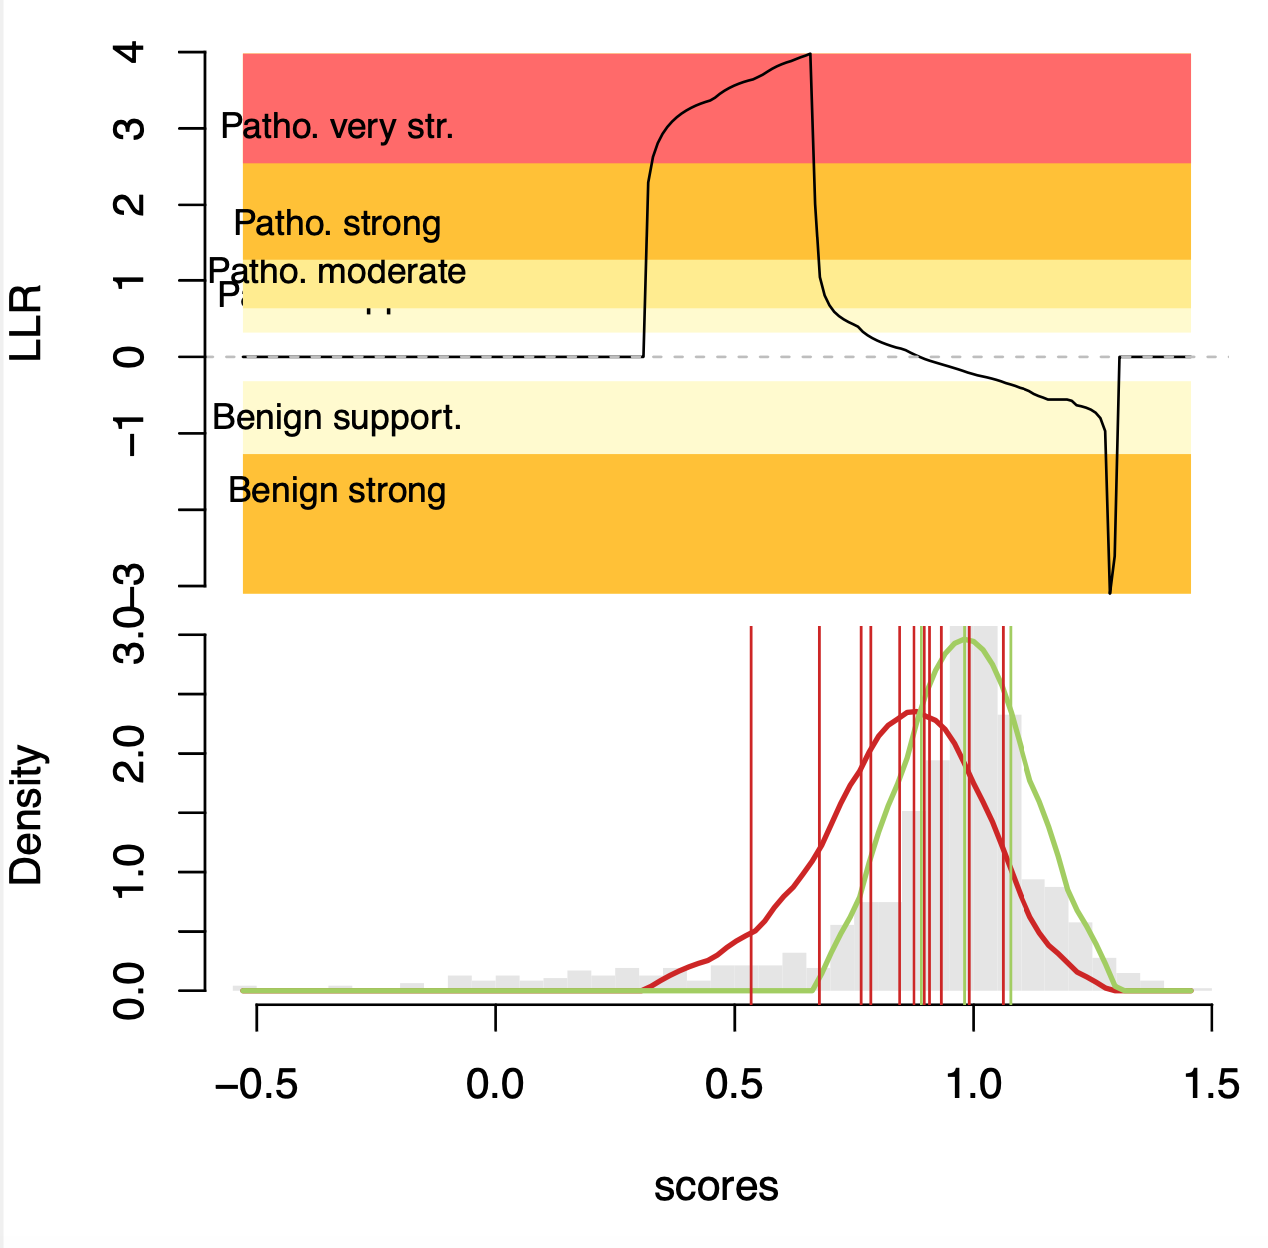
\includegraphics[width=.4\textwidth]{Figures/CALM1/New_LLR.png} }}%
    \qquad
    \subfloat[\centering LLR for 2019 CALM1 map]{{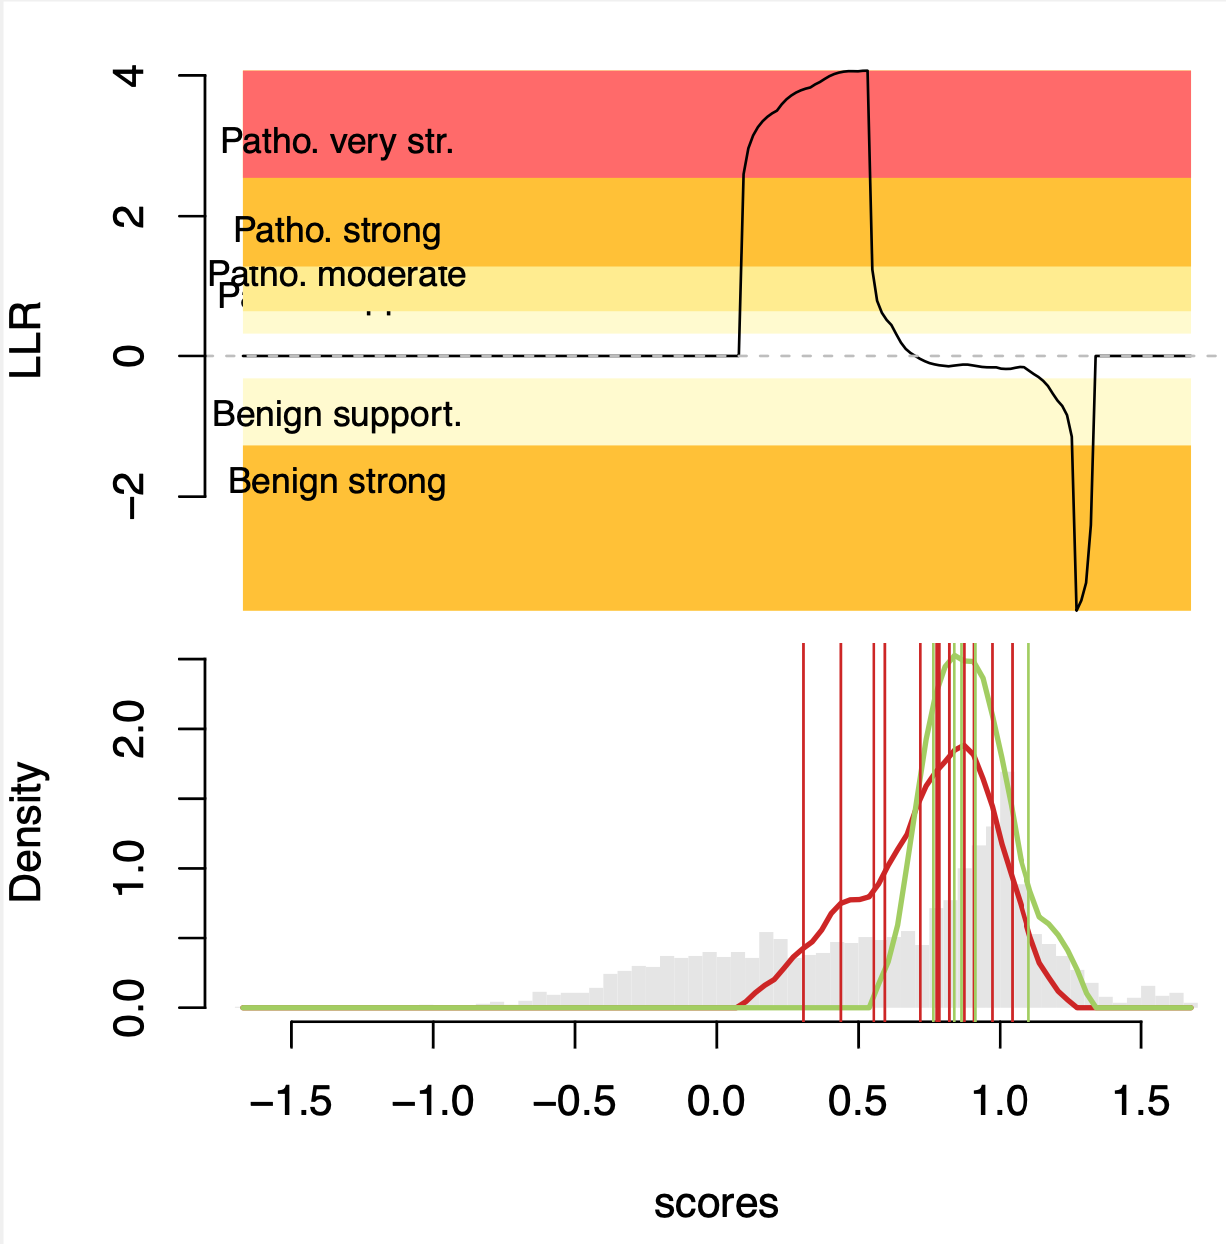
\includegraphics[width=.4\textwidth]{Figures/CALM1/old_LLR.png} }}%
    \caption{The Log-likelihood ratio of pathogenicity for the CALM1 as a function of fitness score.}%
    \label{fig:LLR CALM1}%
\end{figure}


\subsubsection{Comparison between TileSeqPro and the Legacy pipeline}
% se
Similar to the standard error of SUMO1 fitness scores, the standard error of CALM1 fitness scores generated by TileseqPro pipelines have larger standard error than the Legacy version (see supplemental Fig. 7). We also observed that the standard error of the nonsense variants' fitness scores is the highest amongst others.

% \begin{figure}[H]
%     \centering
%     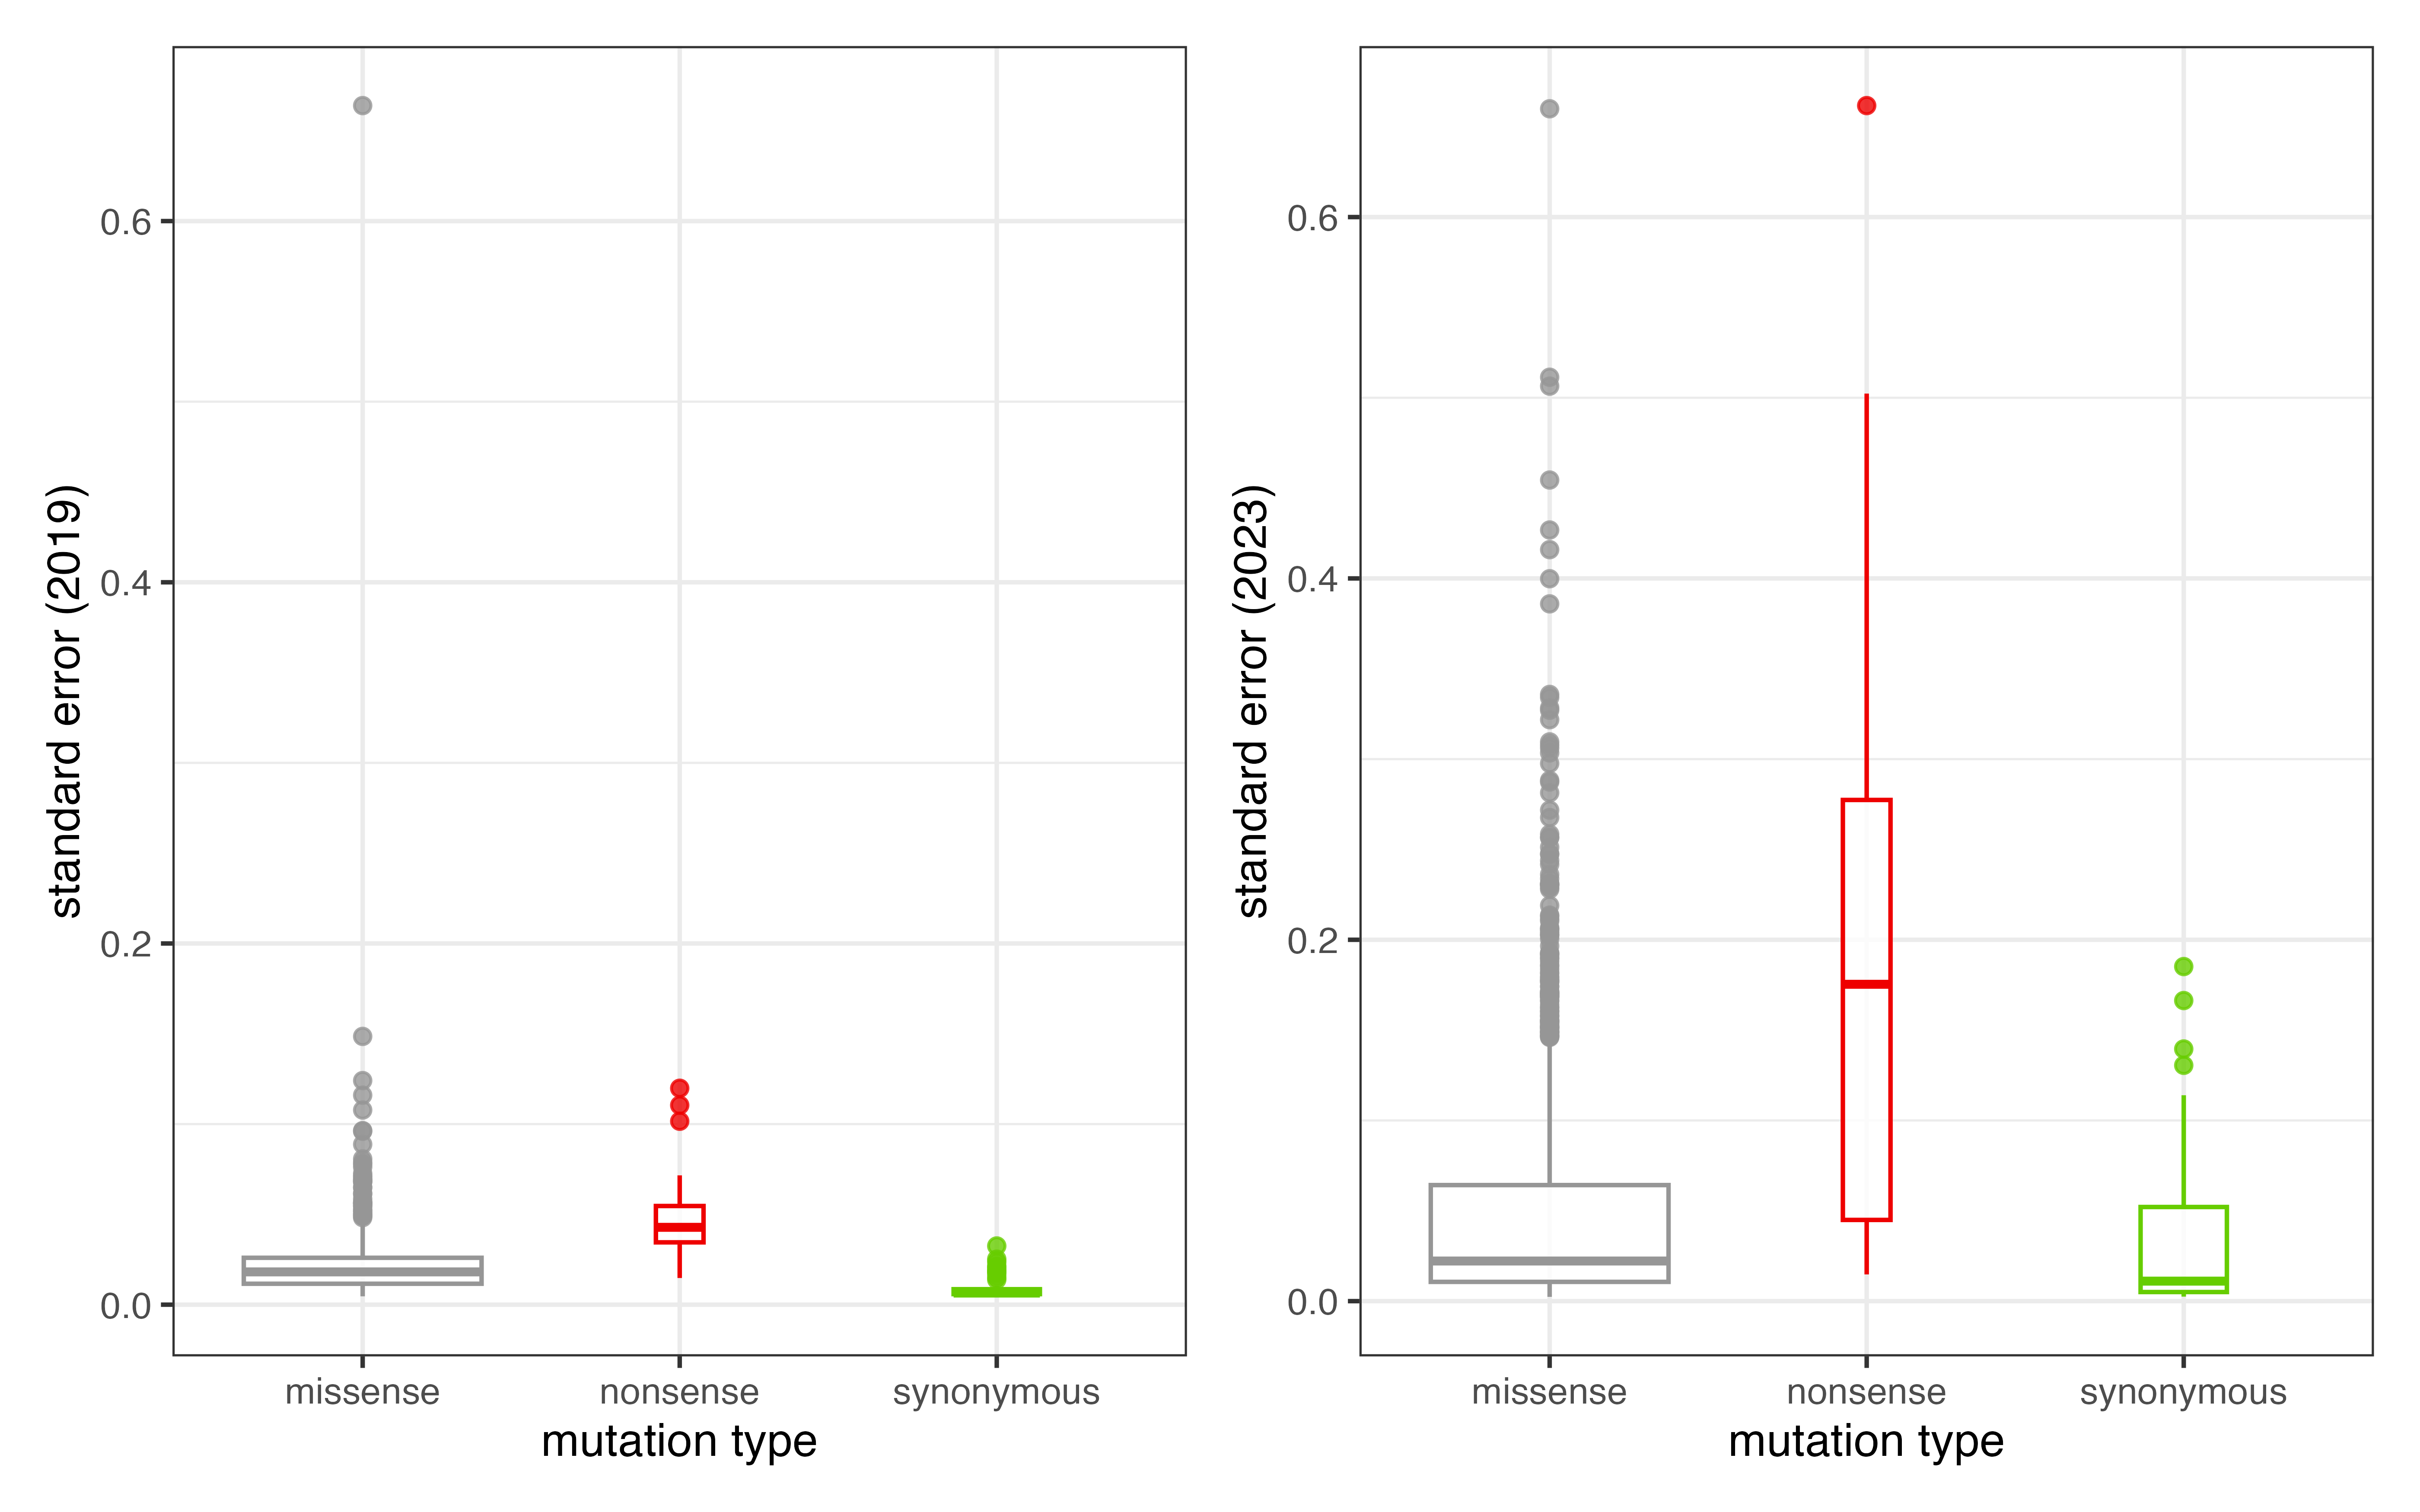
\includegraphics[width =.4\textwidth]{Figures/CALM1/se_boxplot.png}
%     \caption{The distribution of standard error of new and old fitness scores (CALM1).}
%     \label{fig:se boxplot CALM1}
% \end{figure}

% score comparison
The fitness score from the two pipeline versions agrees with each other with a correlation of $\rho = 0.92$ (see supplemental Fig. 8). Nonsense variants have lower correlation ($\rho = 0.59$), compared to missense and synonymous variants ($\rho = 0.91$), likely because nonsense variants have fewer of available amino acid change data and larger standard error. The moving window correlation graph indicates a good correlation from amino acid position 25 to the end, while the correlation for the first 20 amino acid are low because few amino acid changes in that region "survived" after the harsh filtering.


% \begin{figure}[H]%
%     \centering
%     \subfloat[\centering ]{{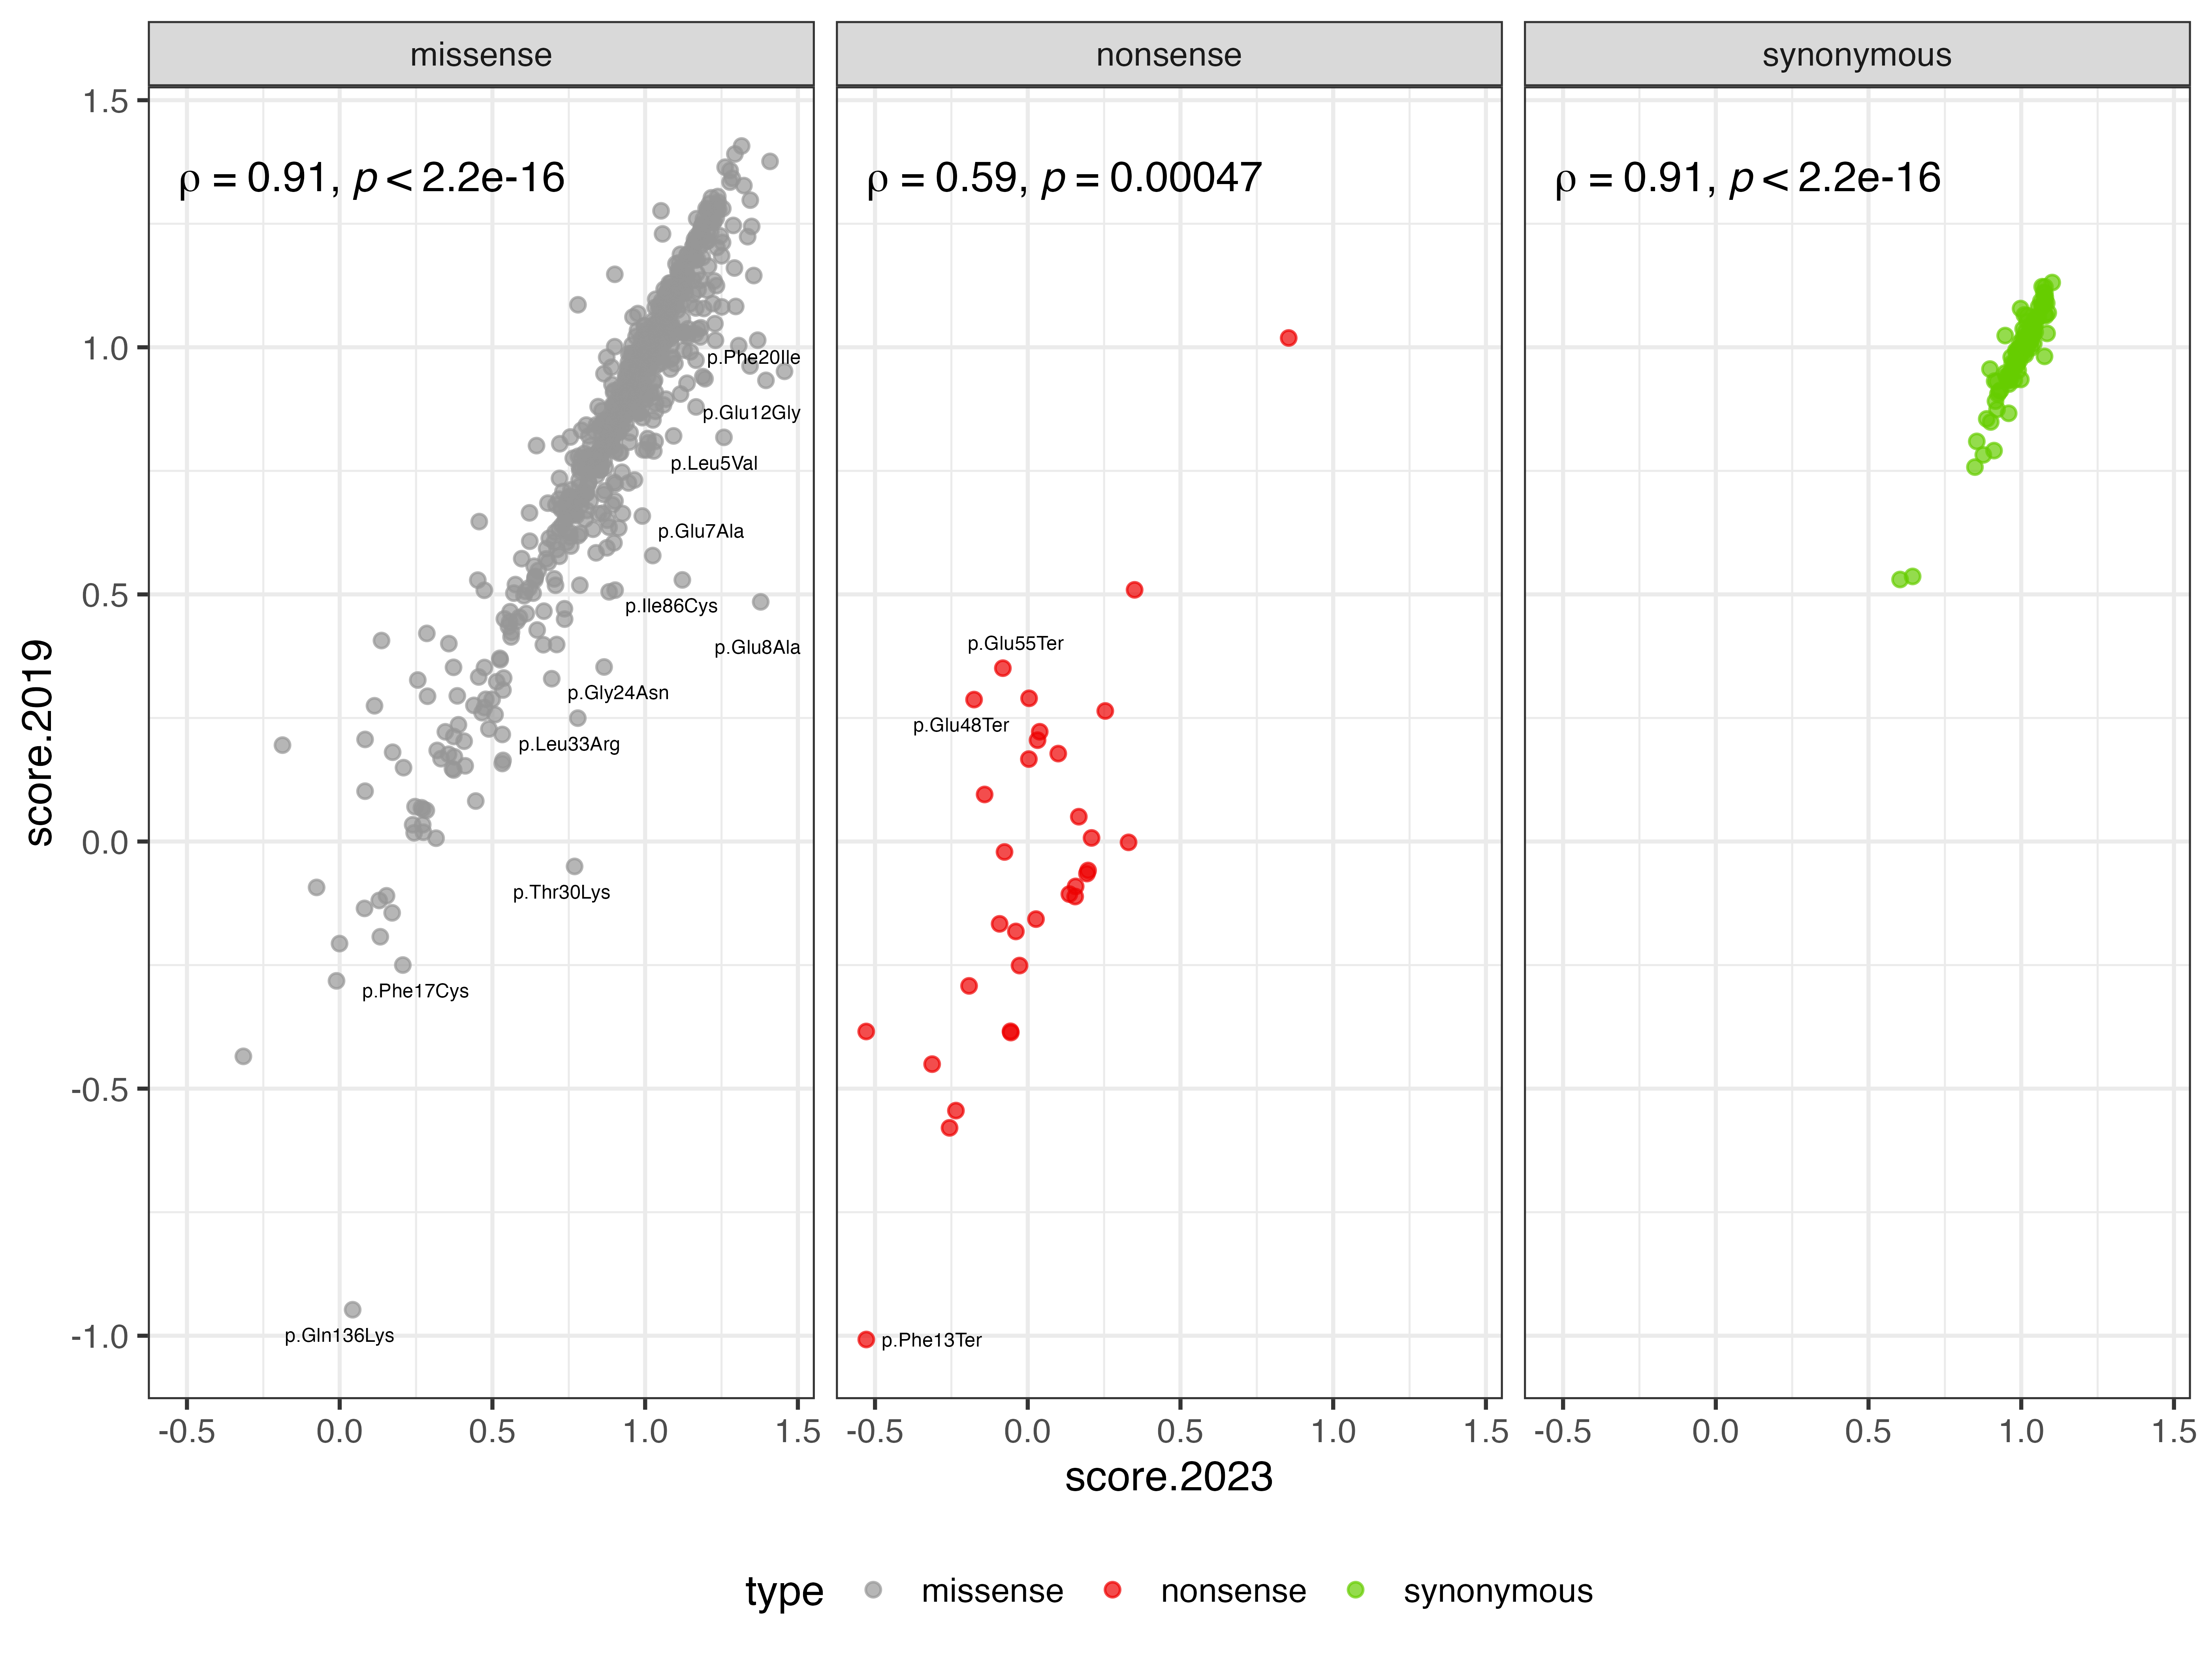
\includegraphics[width=.3\textwidth]{Figures/CALM1/comparison_mutation.png} }}%
%     \qquad
%     \subfloat[\centering ]{{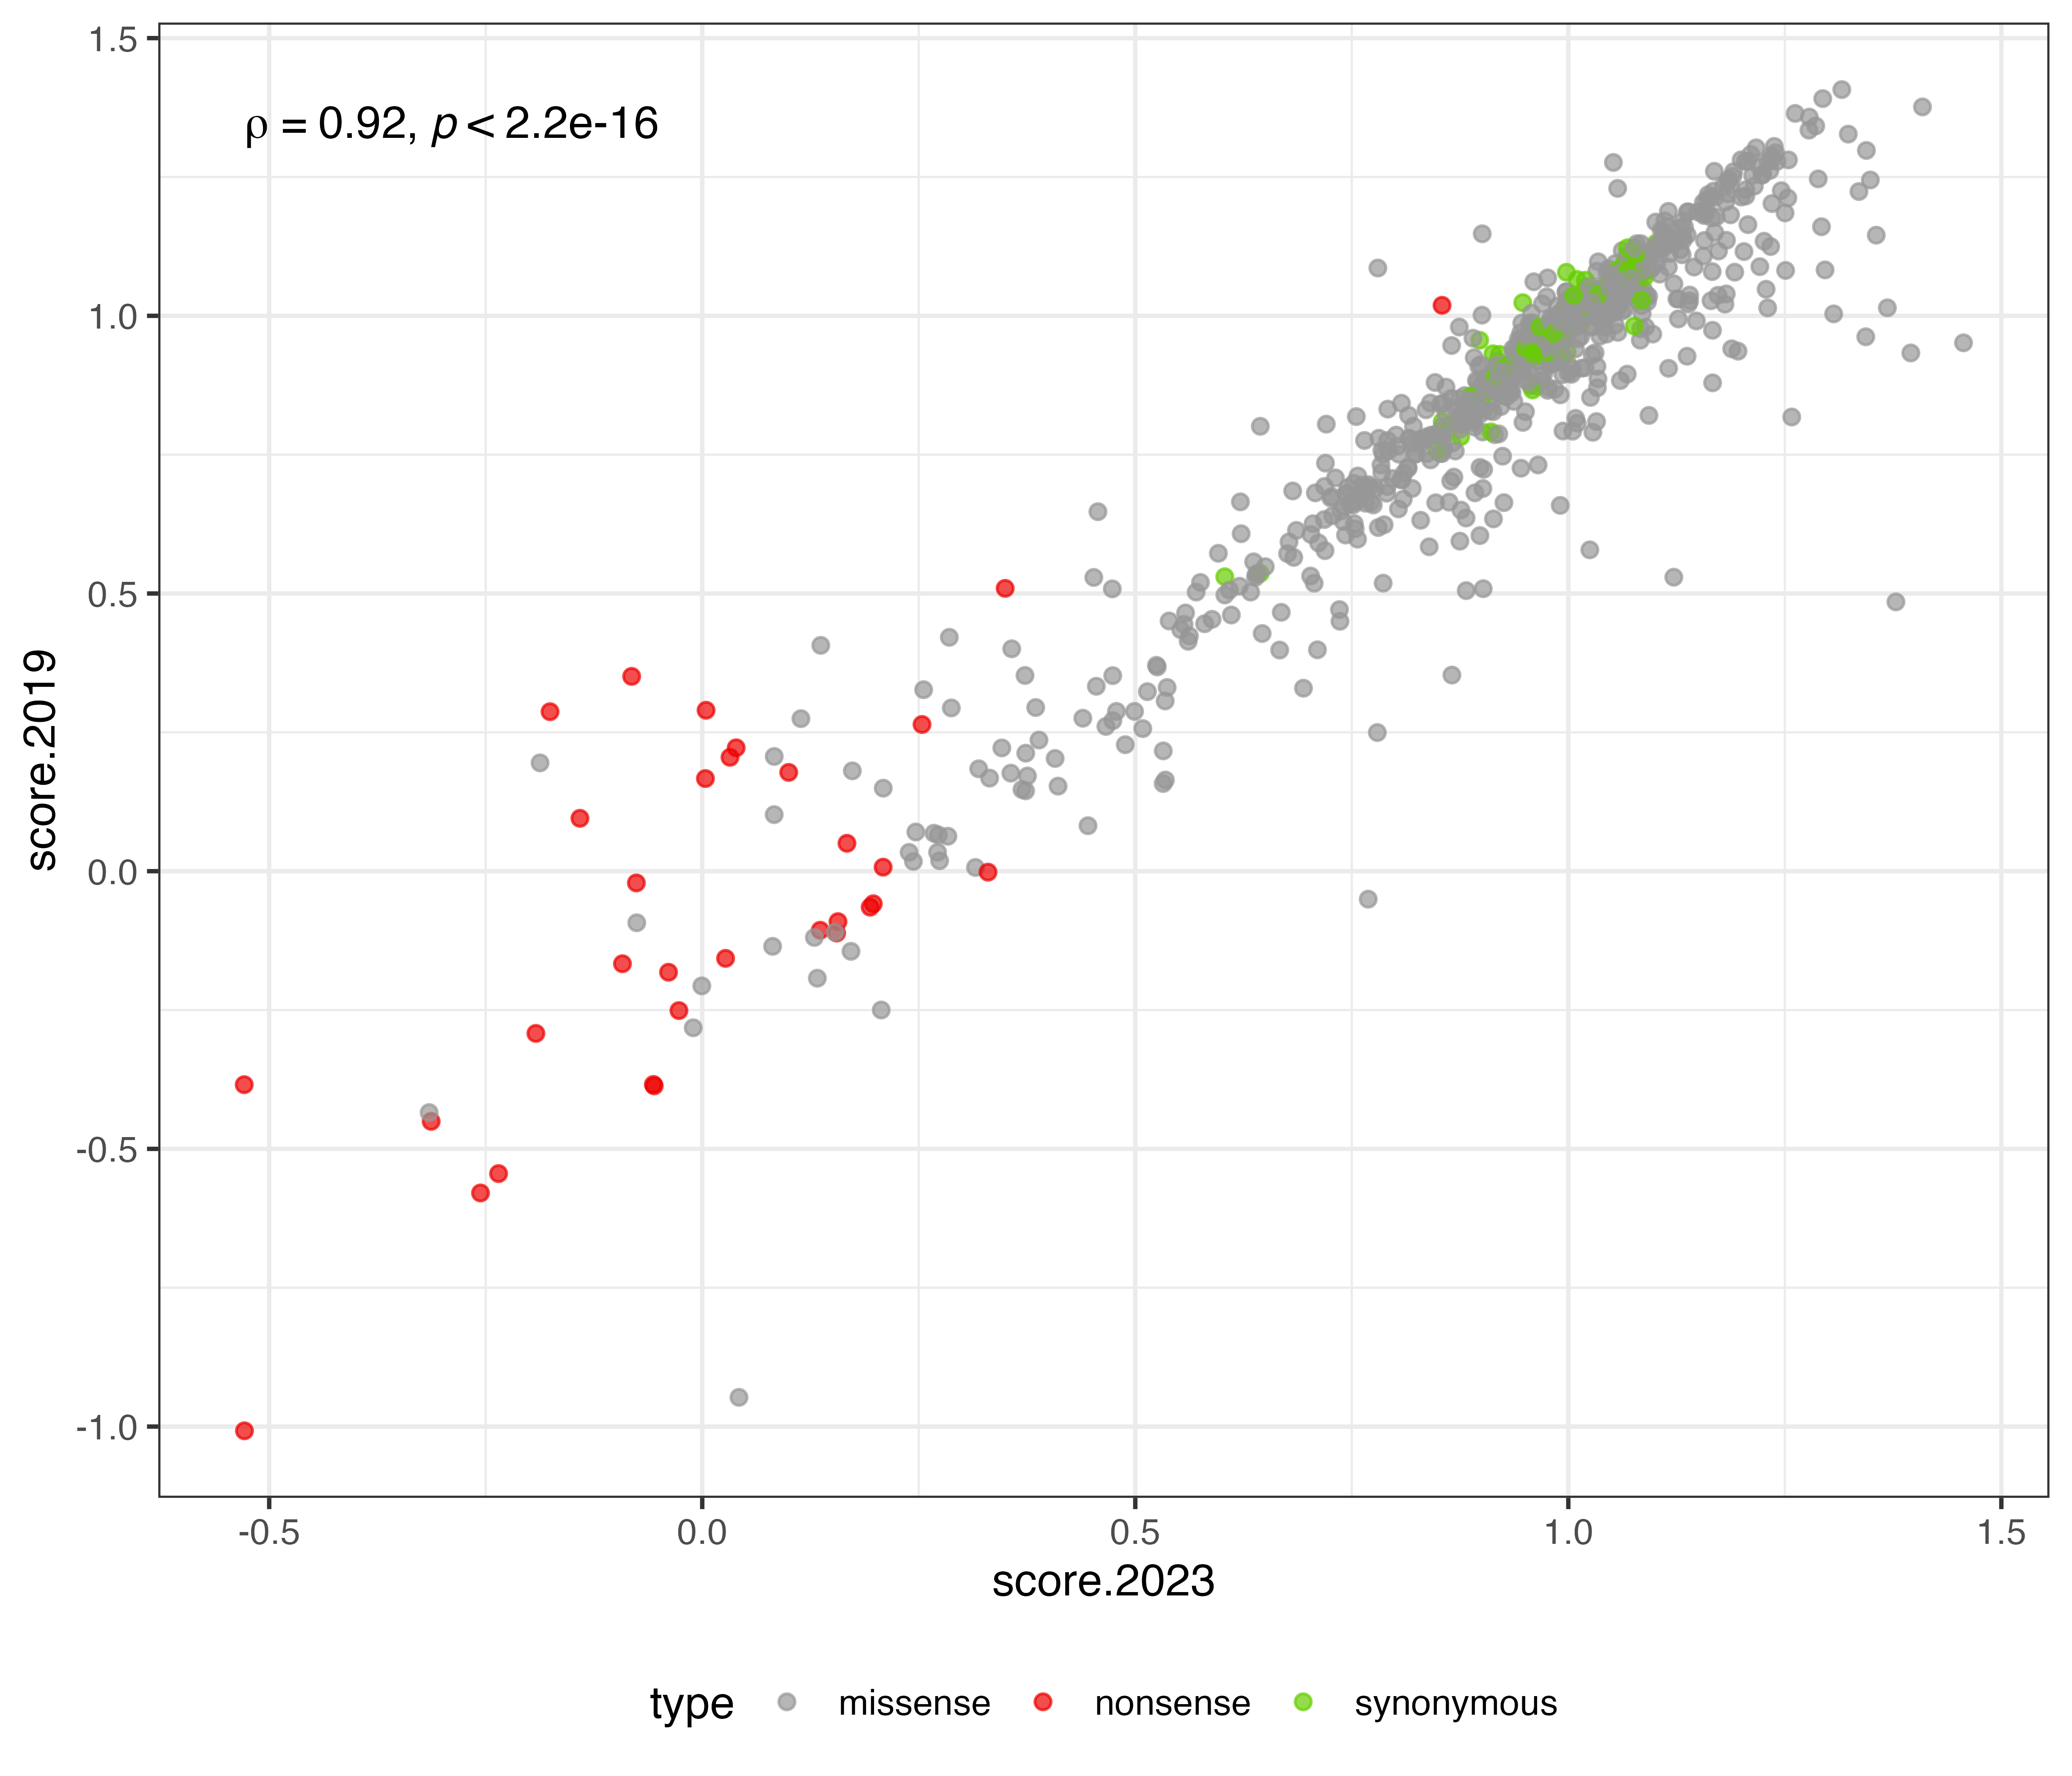
\includegraphics[width=.25\textwidth]{Figures/CALM1/comparison_overall.png} }}%
%     \qquad
%     \subfloat[\centering ]{{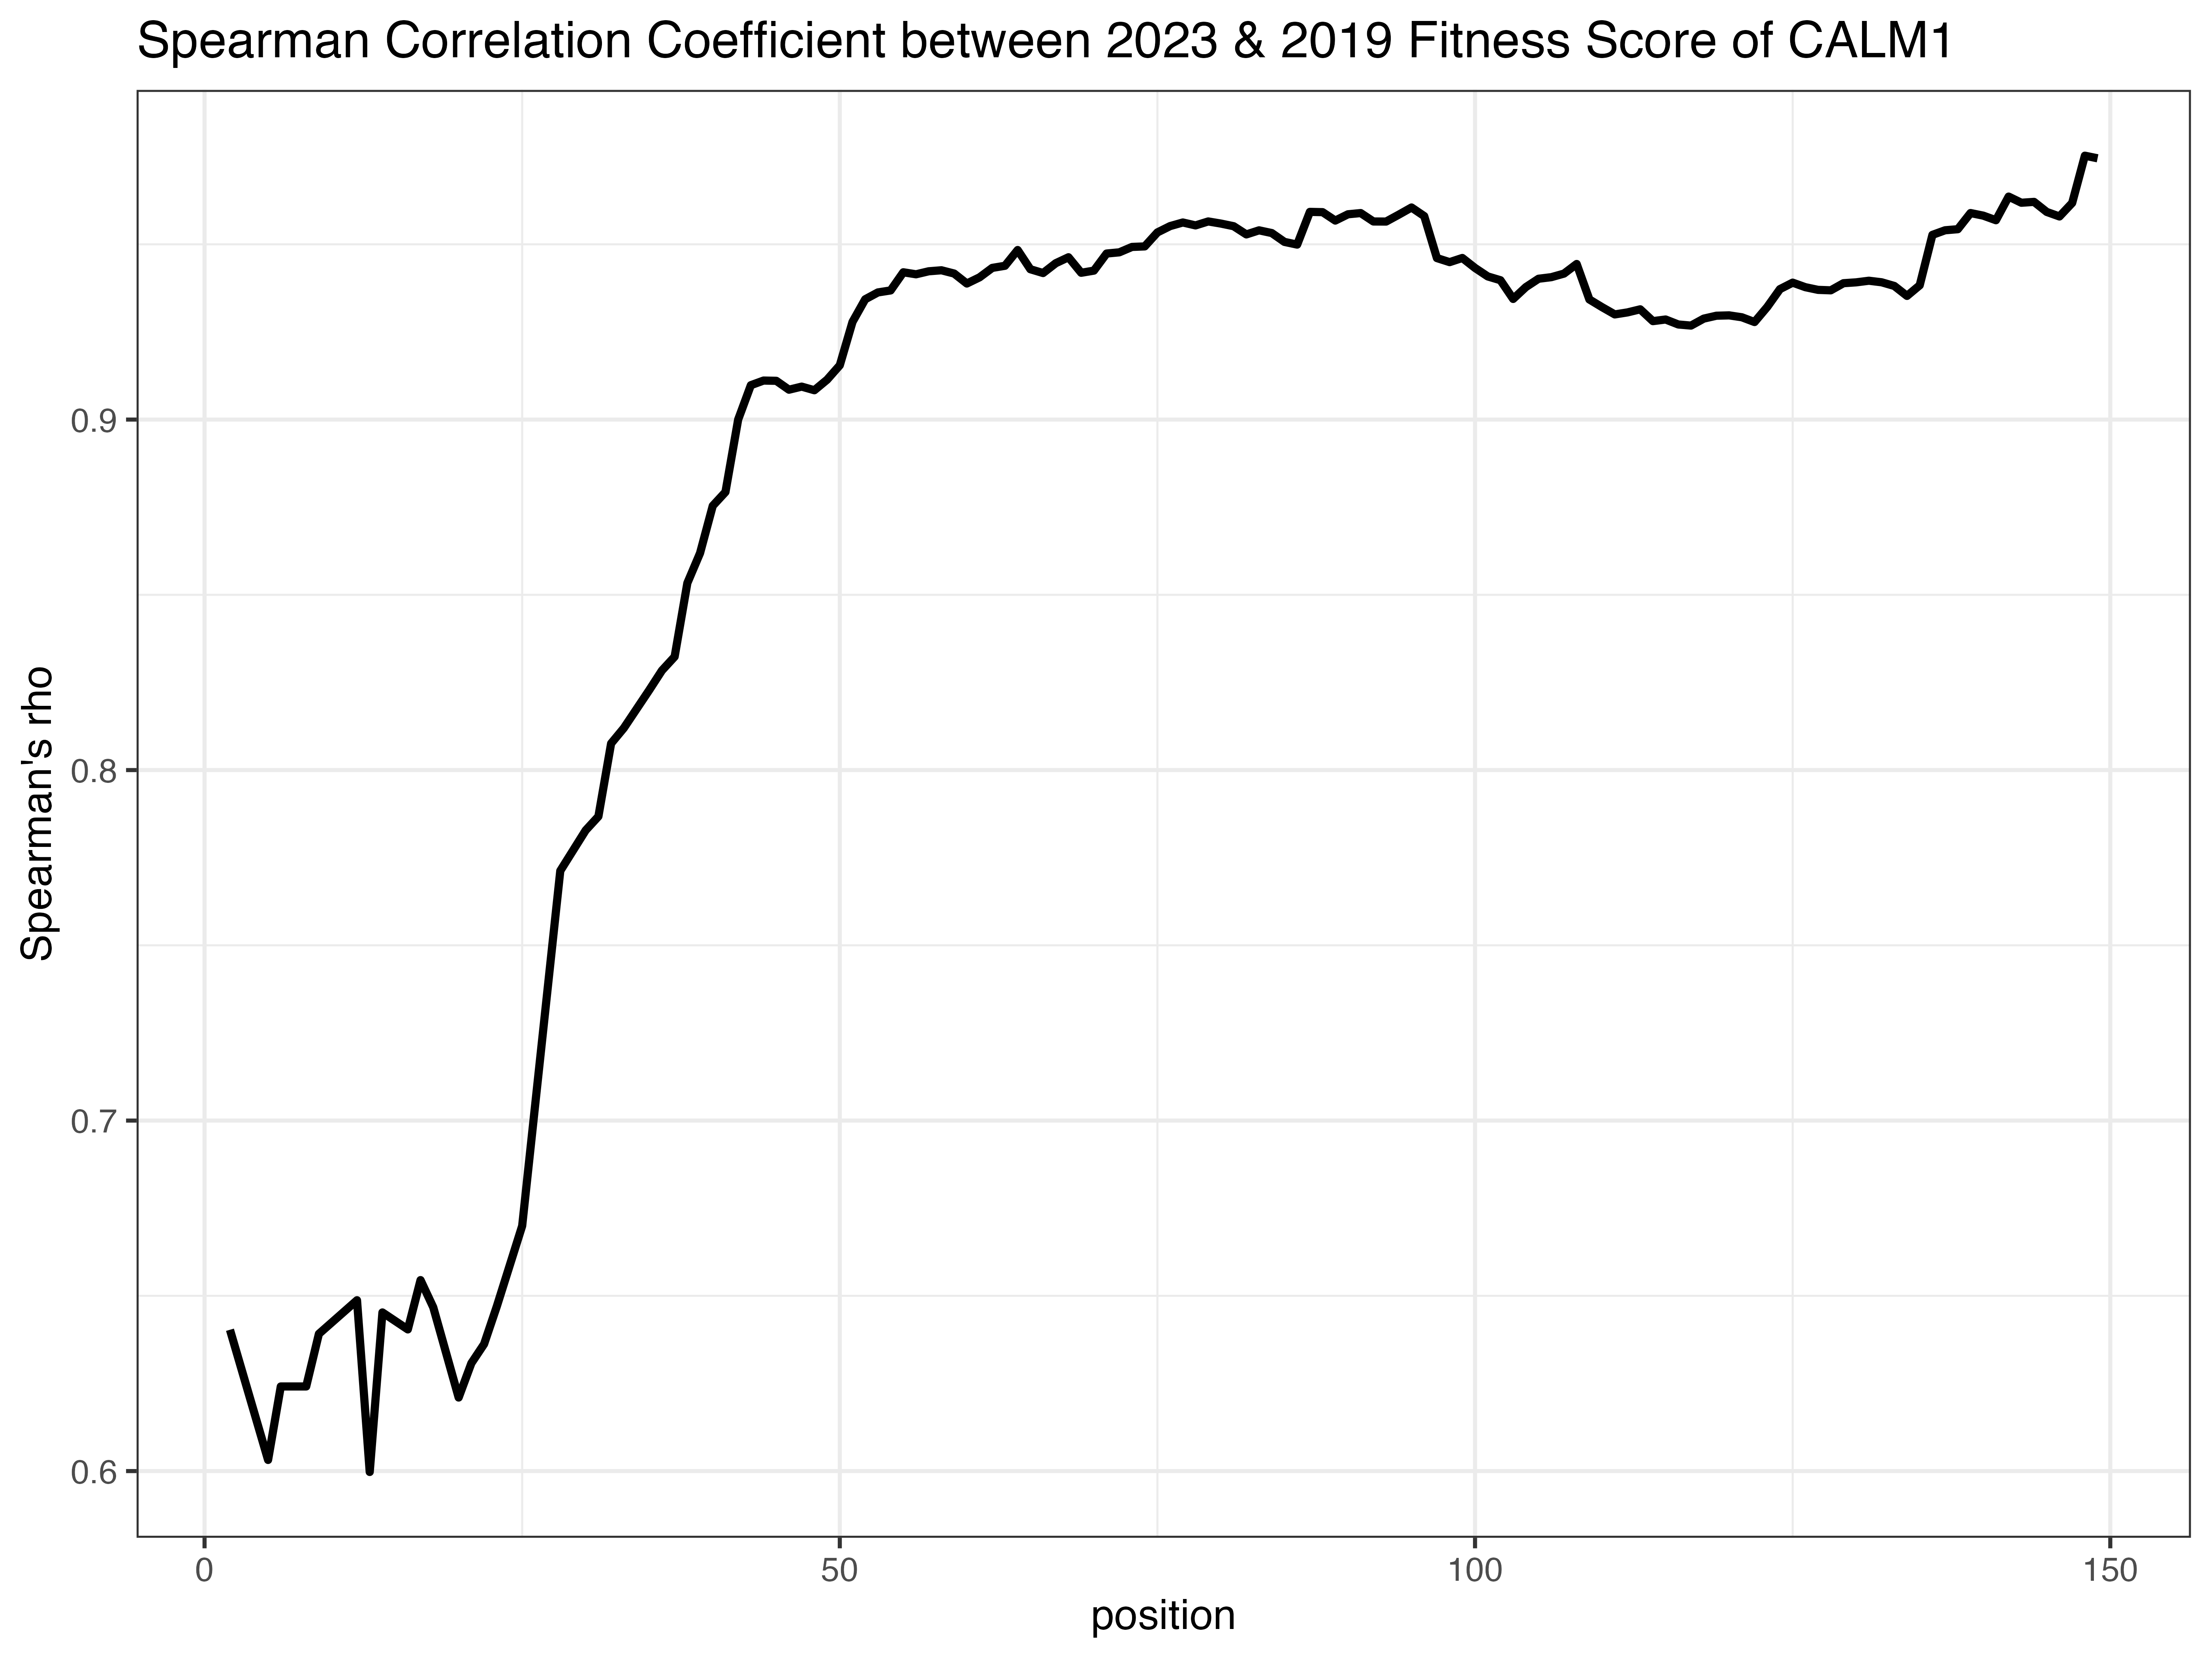
\includegraphics[width=.3\textwidth]{Figures/CALM1/score_rho.png} }}%
%     \caption{(a) and (b) show the scatter plot of fitness scores for CALM1 generated by TileseqPro and Legacy pipelines, (c) is a line graph describing the change of Spearman's correlation between fitness scores along amino acid positions.}%
%     \label{fig:scatter plot CALM1}%
% \end{figure}


\subsubsection{Moving Window Correlation between Fitness Scores and VARITY Scores}
We analyzed the moving window correlation of VARITY scores and fitness scores (Fig. \ref{fig:VARITY_CALM1}). As expected, there is an anti-correlation between these scores. Surprisingly however, the trend of the correlation between fitness scores vs. VARITY\_R and VARITY\_ER are not similar. The Anti-correlation between fitness scores and VARITY\_R are better than with VARITY\_ER. Besides, The anti-correlation between TileseqPro score versus VARITY scores and Legacy scores vs. VARITY scores are similar, despite the region around the first twenty amino acids.


\begin{figure}[H]%
    \centering
    \subfloat[\centering Correlation between VARITY\_R Scores and Fitness Scores]{{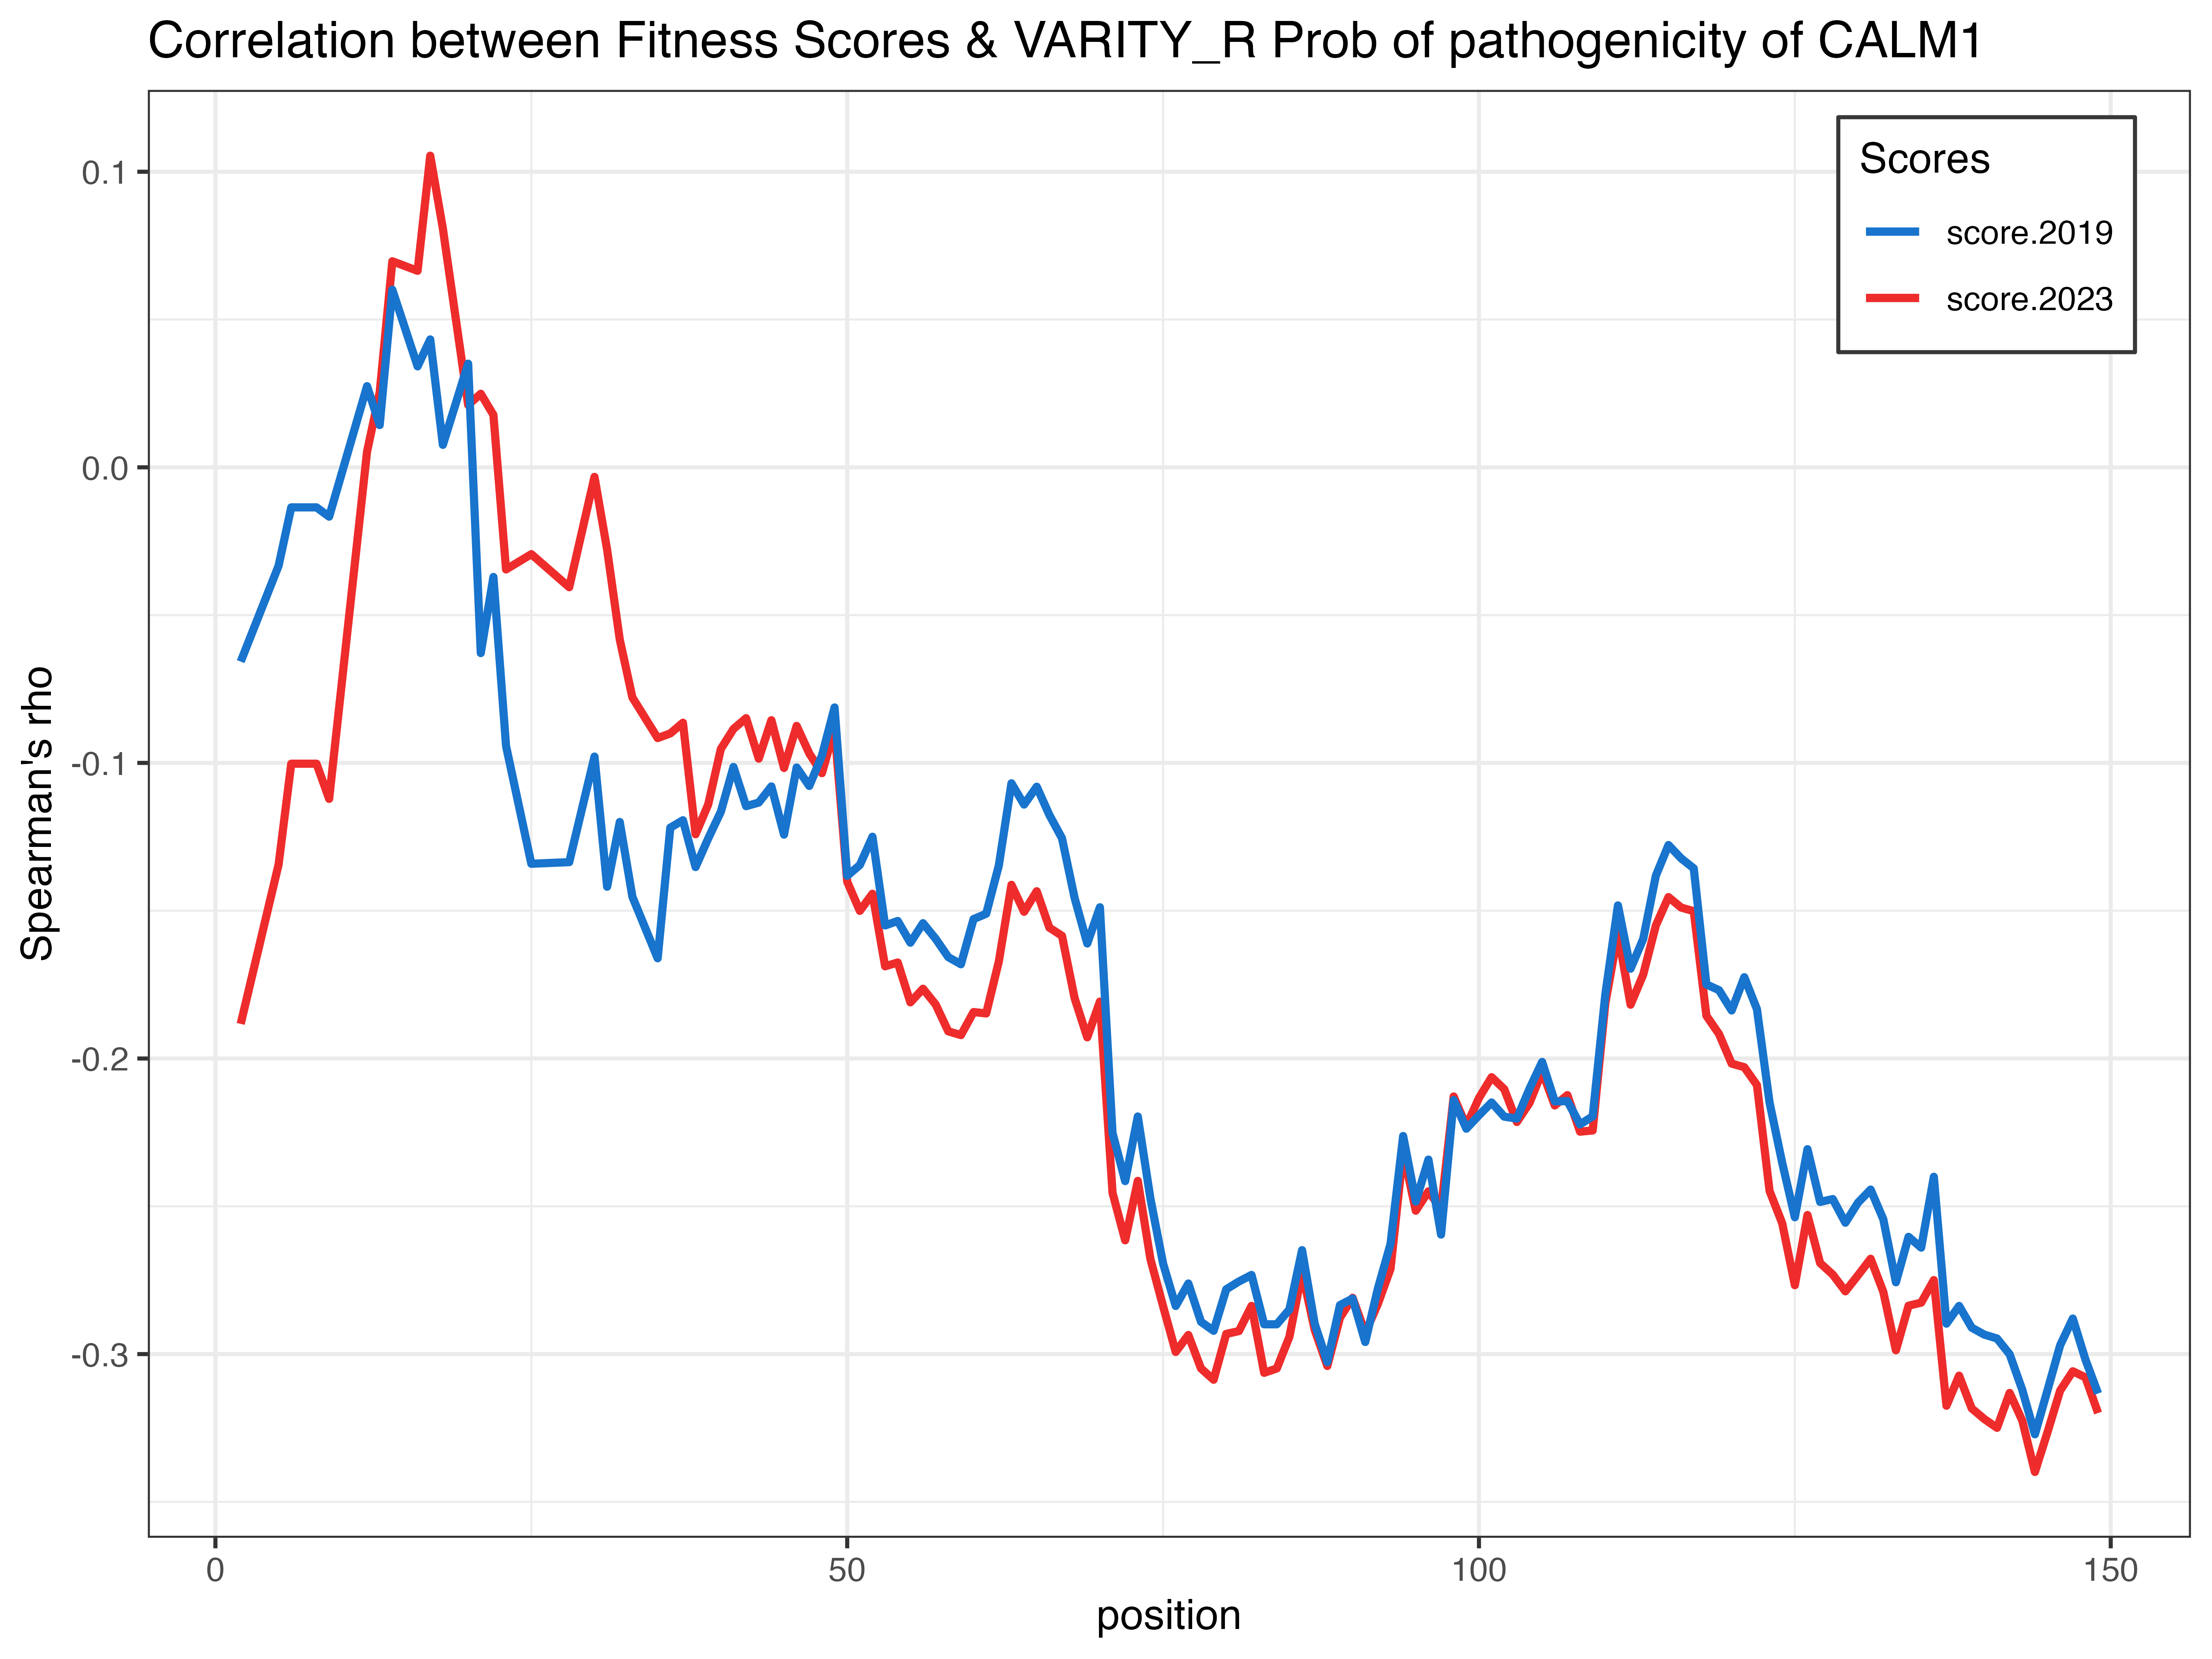
\includegraphics[width=.45\textwidth]{Figures/CALM1/spearman_VARITY_R.png} }}%
    \qquad
    \subfloat[\centering Correlation between VARITY\_ER Scores and Fitness Scores]{{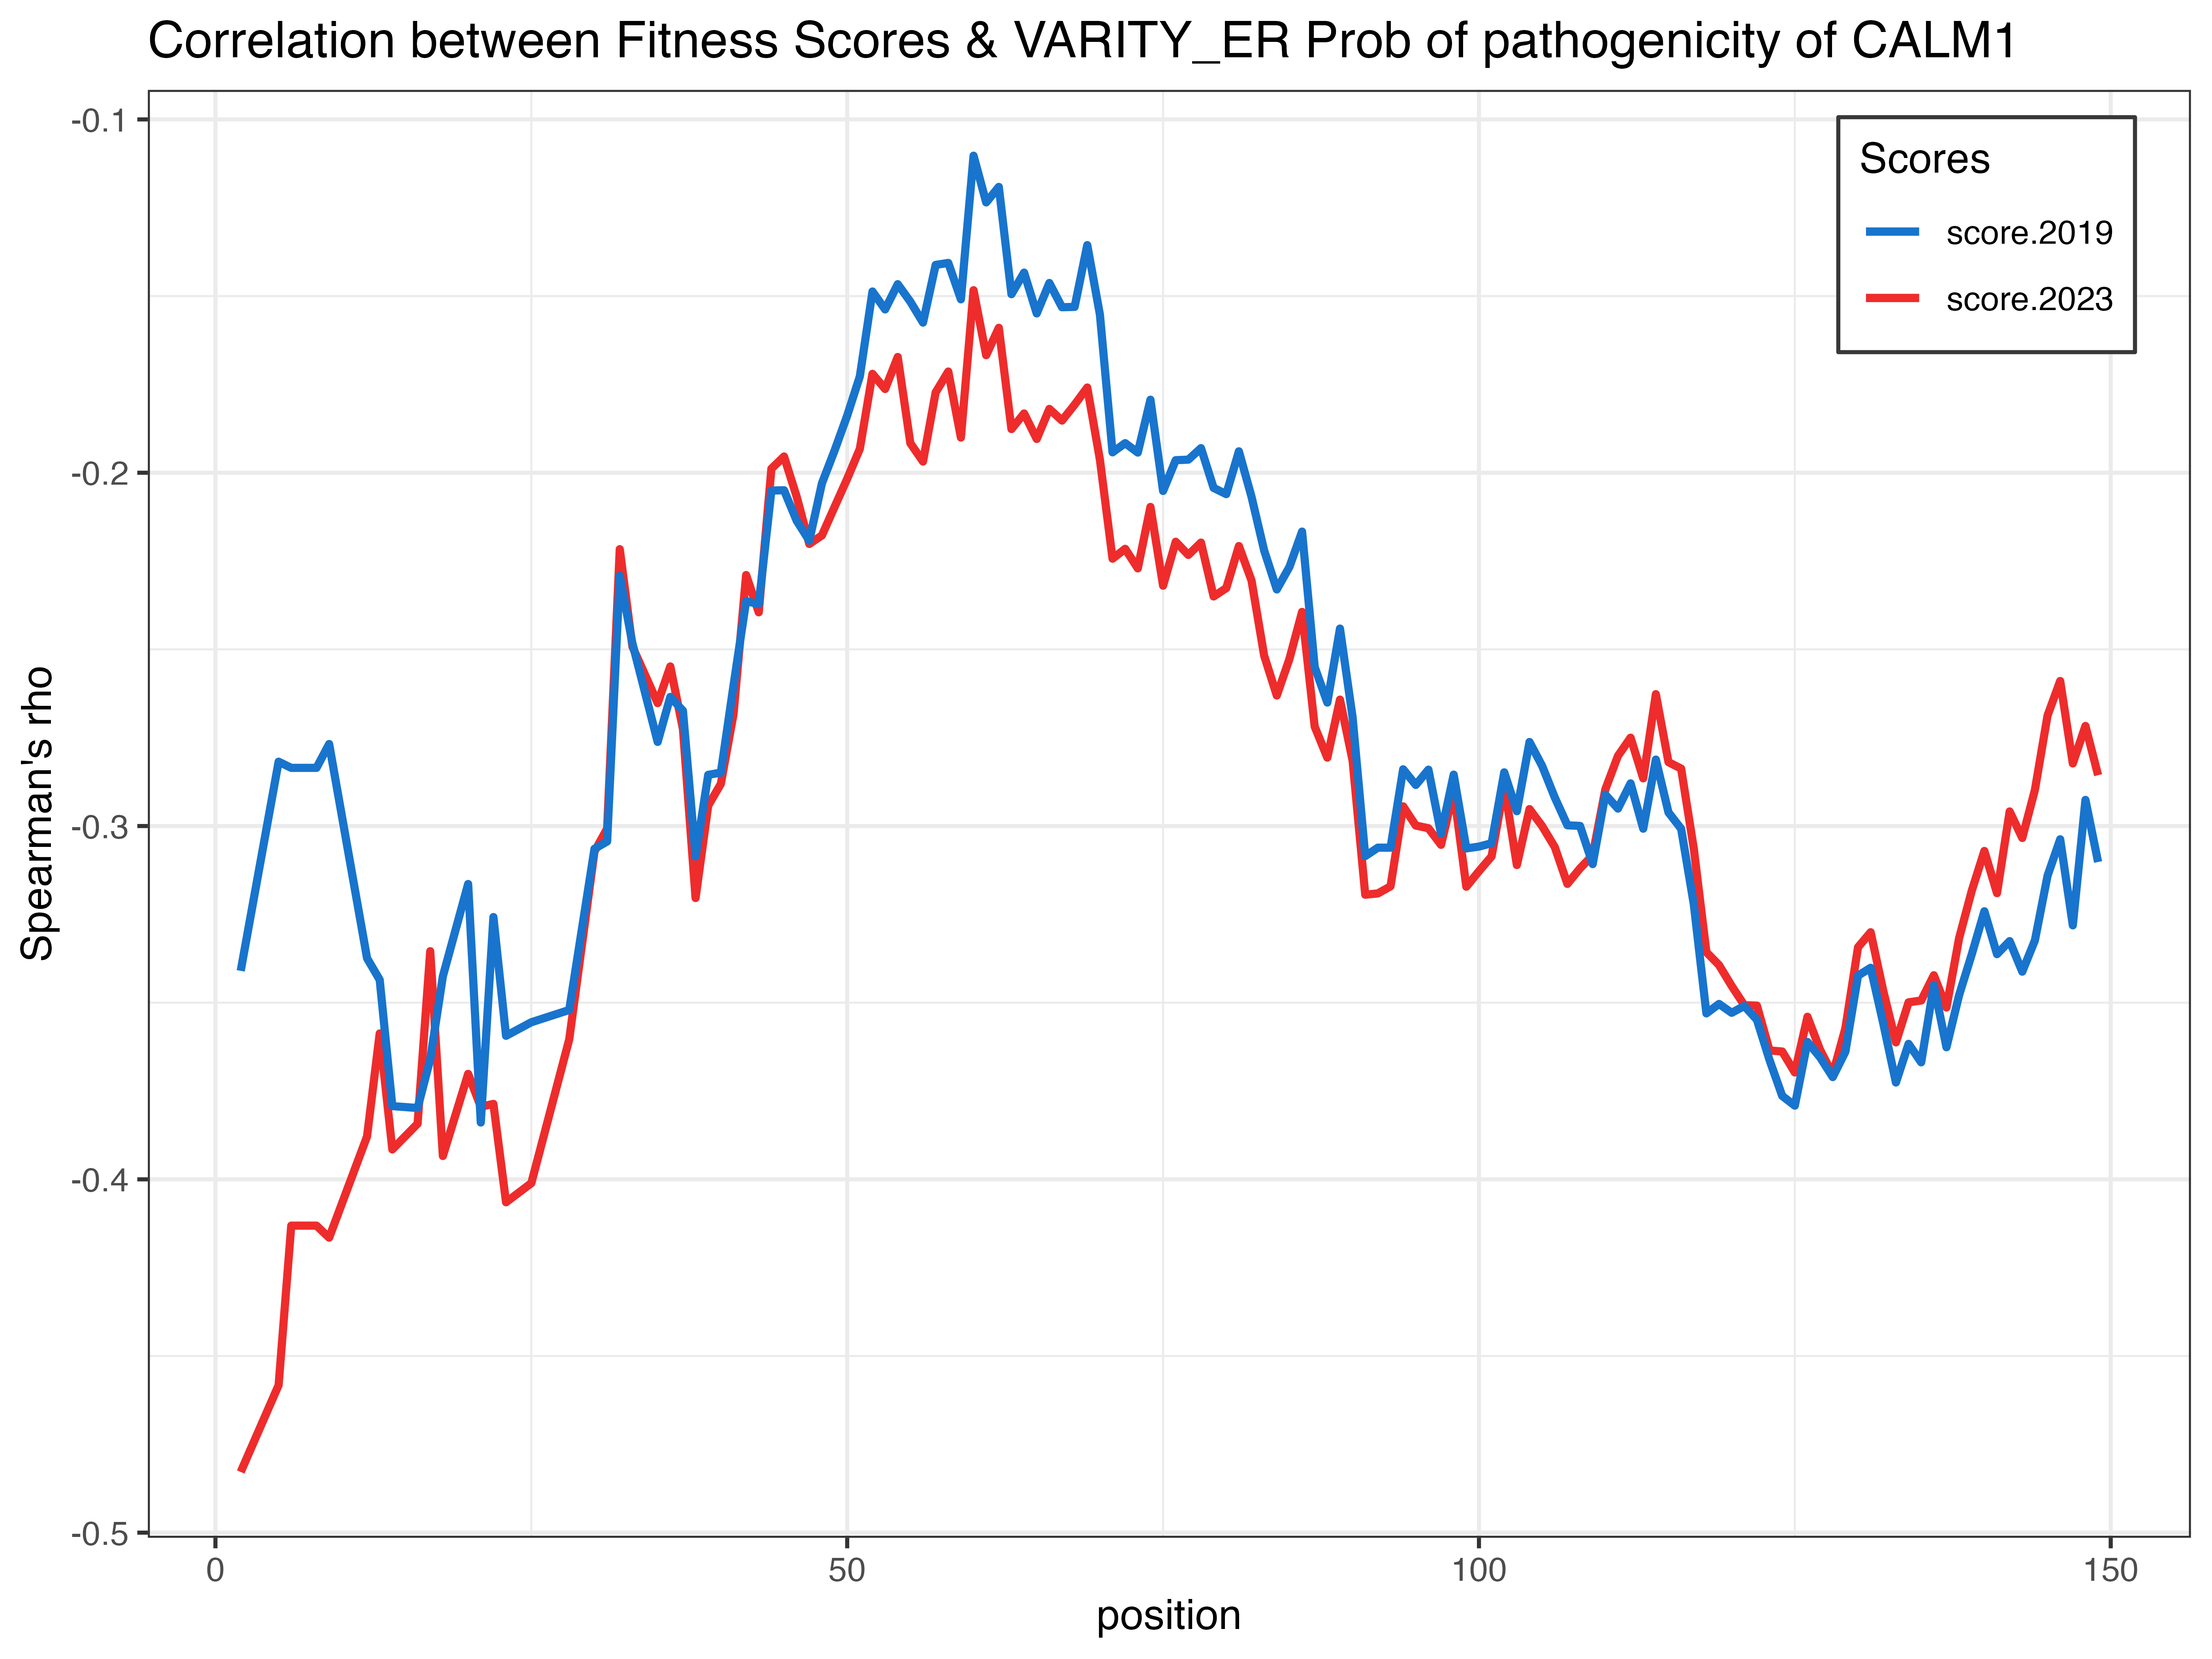
\includegraphics[width=.45\textwidth]{Figures/CALM1/spearman_VARITY_ER.png} }}%
    \caption{Moving window correlation between VARITY Scores and Fitness Scores. Blue line represents the old scores, and red line represents the updated scores.}%
    \label{fig:VARITY_CALM1}%
\end{figure}


\subsubsection{Conclusion}
Though we threw out lots of codon changes with low marginal frequencies when re-calculating the map with TileseqPro, the newer version of CALM1 map performed better in terms of gaining more precision. There is still a high correlation between both versions of CALM1 fitness scores, and the anti-correlation between VARITY scores and both version of fitness scores look similar.


\subsection{MTHFR}
We also re-processed maps for MTHFR\cite{weile_shifting_2021}. The original maps were measured in two different genetic backgrounds (WT and A222V) and at four different concentrations of folinic acid (12 $\mu$g/ml (f12AV), 25 $\mu$g/ml (f25AV), 100 $\mu$g/ml (f100AV) to 200 $\mu$g/ml (f200AV)). Here we completed reprocessing of the four maps in the A222V background. The MTHFR variant effect maps currently deposited on MaveDB were first calculated in 2019, and last updated by 2020.

\subsubsection{Observations from QC results}
The MTHFR map was subdivided into four separate mutagenesis regions, which show an extrapolated average number of 0.941, 0.769, 0.864, and 0.791 amino acid changes per clone, respectively (see supplemental Fig. 10). Accordingly, the overall coverage presented by the coverage heatmap (see supplemental Fig. 9) appears low, with lots of low-frequency variants, especially in Tiles 10, 18, and 19.

Inspecting the distribution of nonsense and synonymous variant enrichment ratios ($\log(\phi)$) relative to marginal frequency thresholds at different folate concentrations (see supplemental Fig. 11), we observed that the separation between enrichment values improved at a frequency of ${10}^{-4.6}$. Given the sequencing depth of 2M reads per sample, we chose a count threshold at 50 corresponding to this observation. After setting filters using this setting, around half of variants were filtered out by the frequency and bottleneck filter.

Following the filtering steps, there is a relatively clear separation between the enrichment values of nonsense and synonymous MTHFR variants (Fig. \ref{fig:enrichment MTHFR}) at four folate concentrations, with the 200 $\mu g / ml$ folinate condition showing the best separation. The mode of nonsense variants is located around $\log(\phi)=-0.8$, and the mode for synonymous variants is located around -0.03 for region all. However, the modes vary a lot by regions: $\log(\phi)=-0.85$ for nonsense variants and $\log(\phi)=-0.023$ for synonymous variants in Region 1; $\log(\phi)=-1.17$ for nonsense variants and $\log(\phi)=0.084$ for synonymous variants in Region 2; $\log(\phi)=-1.2$ for nonsense variants and $\log(\phi)=-0.23$ for synonymous variants in Region 3; and $\log(\phi)=-0.542$ and $\log(\phi)=-0.04$ for nonsense and synonymous variants in Region 4, respectively. The missense variants have only one mode near 0, indicating most missense variants of MTHFR have relatively mild fitness effects.

\begin{figure}[H]%
    \centering
    \subfloat[\centering f12AV]{{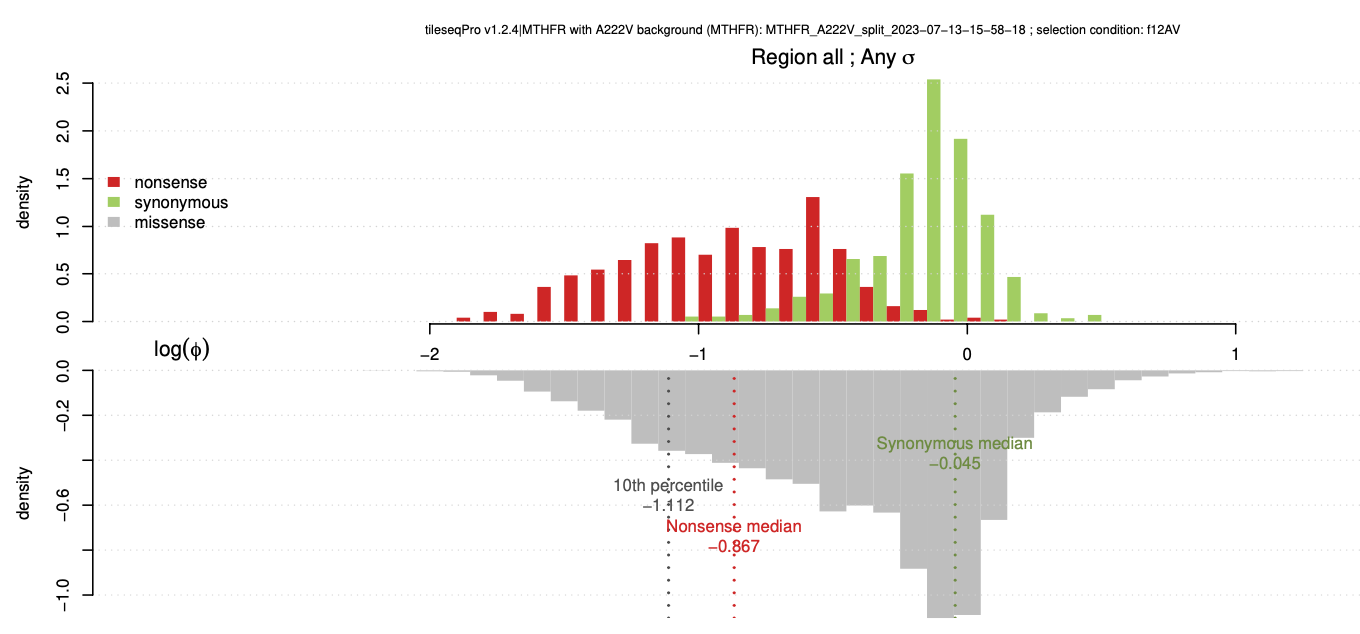
\includegraphics[width=.45\textwidth]{Figures/MTHFR/f12AV_BCE.png} }}%
    \qquad
    \subfloat[\centering f25AV]{{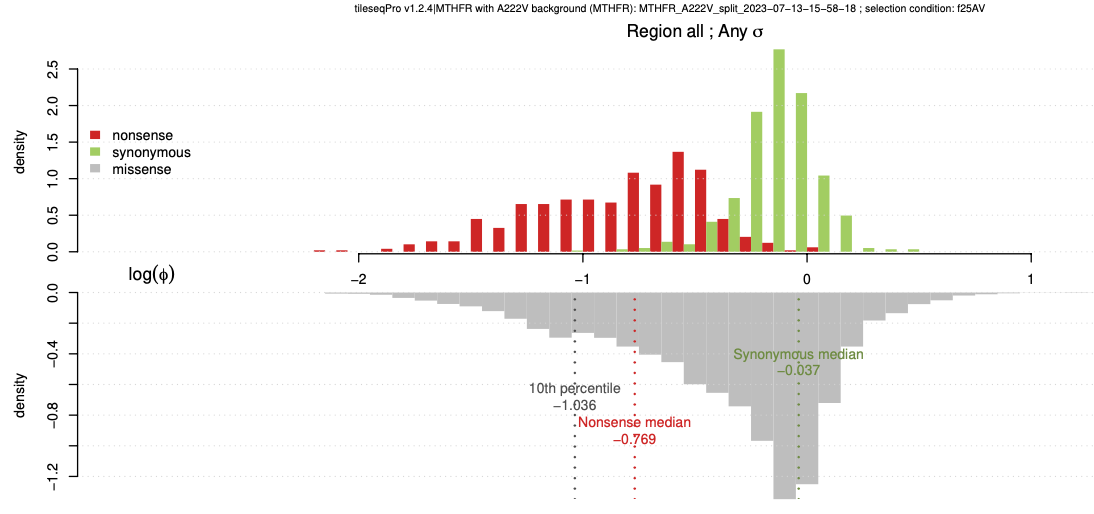
\includegraphics[width=.45\textwidth]{Figures/MTHFR/f25AV_BCE.png} }}%
    \qquad
    \subfloat[\centering f100AV]{{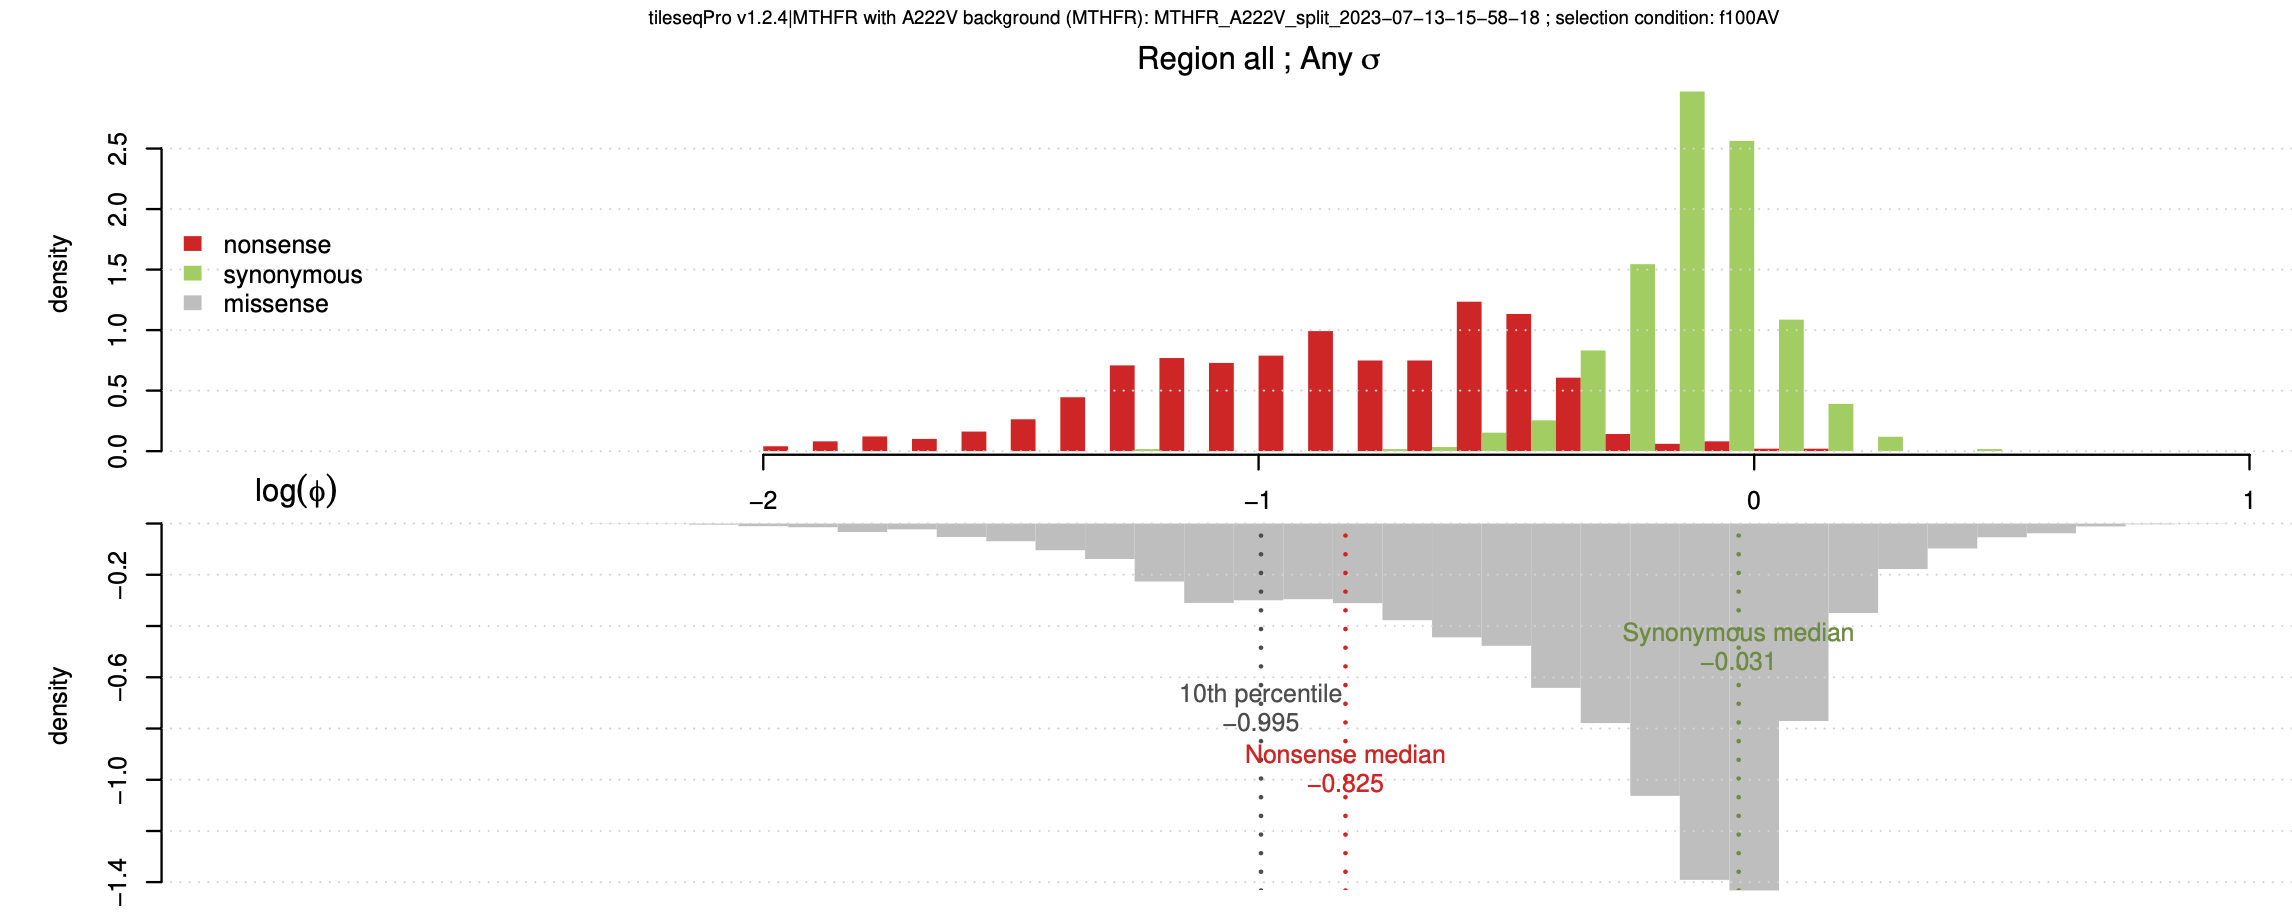
\includegraphics[width=.45\textwidth]{Figures/MTHFR/f100AV_BCE.png} }}%
    \qquad
    \subfloat[\centering f200AV]{{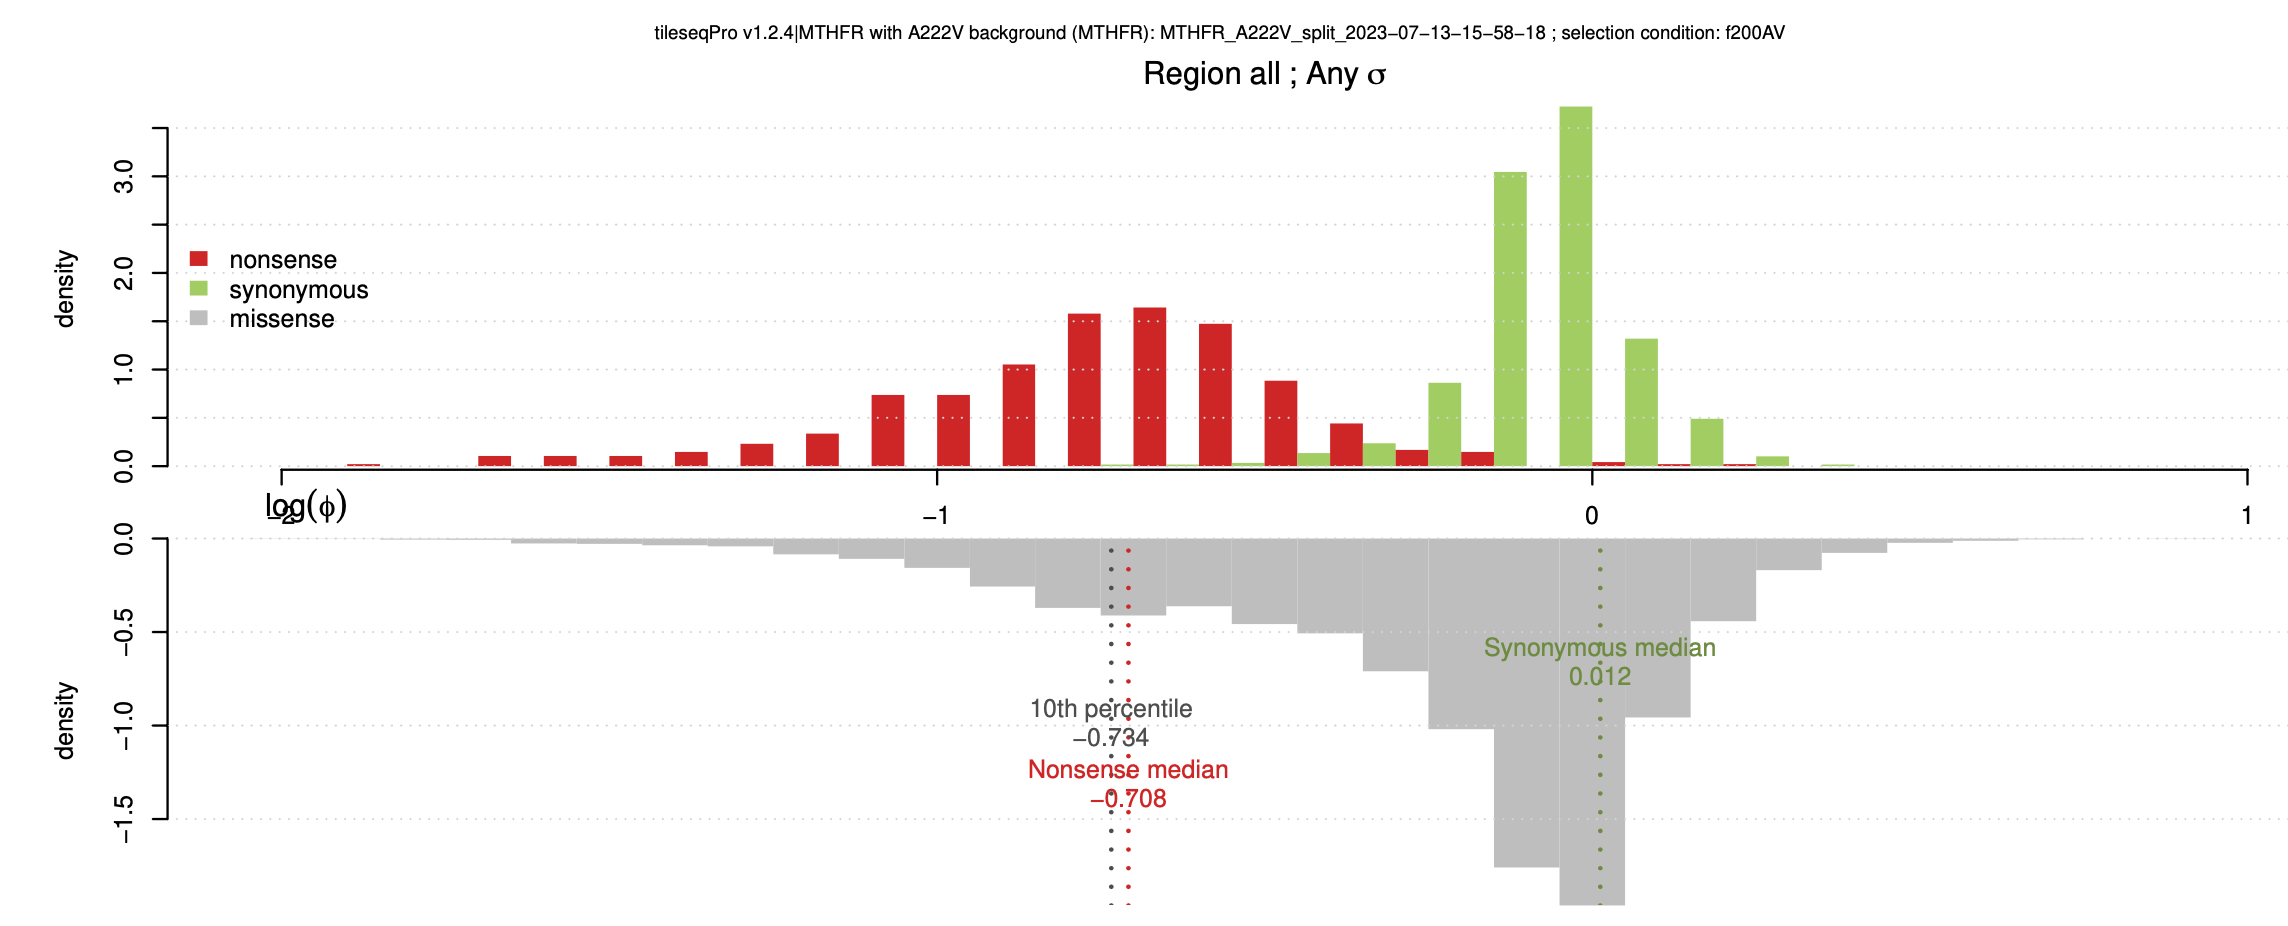
\includegraphics[width=.45\textwidth]{Figures/MTHFR/f200AV_BCE.png} }}%
    \caption{enrichment value distribution of MTHFR variants in A222V background, separated by different folate concentrations.}%
    \label{fig:enrichment MTHFR}%
\end{figure}



A comparison between the MTHFR variant effect maps calculated by TileseqPro and the Legacy pipelines is shown in Figure \ref{fig:new MTHFR map} and \ref{fig:old MTHFR map}. The comparison is complicated by the fact that the maps for f12AV, f25AV, and f100AV available on MaveDB were previously "flipped and floored", i.e. any variants with scores above 1 were inverted by a $f(x)=\frac{1}{x}$ operation and scores below zero were set to exactly zero. This is visible especially in the serine-rich region and regulatory domain, where the maps calculated by TileseqPro pipelines show hypercomplementing variants which are not visible in the MaveDB map.


\begin{figure}[H]%
    \centering
    \subfloat[\centering f12AV]{{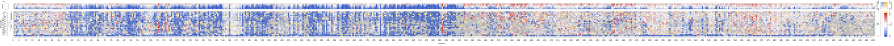
\includegraphics[width=.95\textwidth]{Figures/MTHFR/f12AV_new.png} }}%
    \qquad
    \subfloat[\centering f25AV]{{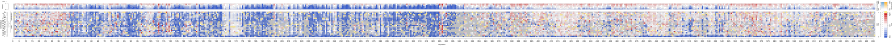
\includegraphics[width=.95\textwidth]{Figures/MTHFR/f25AV_new.png} }}%
    \qquad
    \subfloat[\centering f100AV]{{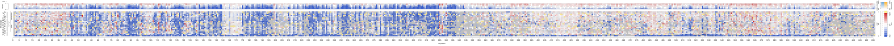
\includegraphics[width=.95\textwidth]{Figures/MTHFR/f100AV_new.png} }}%
    \qquad
    \subfloat[\centering f200AV]{{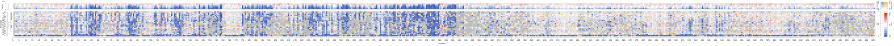
\includegraphics[width=.95\textwidth]{Figures/MTHFR/f200AV_new.png} }}%
    \caption{Mavevis heatmaps for MTHFR variants in A222V background calculated by TileseqPro pipelines, separated by different folate concentrations.}%
    \label{fig:new MTHFR map}%
\end{figure}

\begin{figure}[H]%
    \centering
    \subfloat[\centering f12AV]{{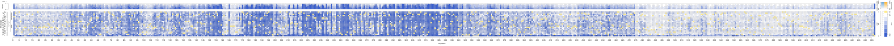
\includegraphics[width=.95\textwidth]{Figures/MTHFR/MAVE_f12AV.png} }}%
    \qquad
    \subfloat[\centering f25AV]{{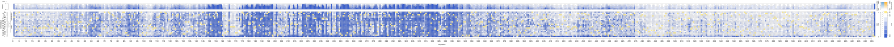
\includegraphics[width=.95\textwidth]{Figures/MTHFR/MAVE_f25AV.png} }}%
    \qquad
    \subfloat[\centering f100AV]{{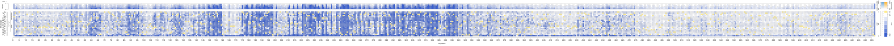
\includegraphics[width=.95\textwidth]{Figures/MTHFR/MAVE_f100AV.png} }}%
    \qquad
    \subfloat[\centering f200AV]{{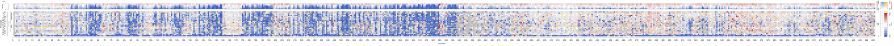
\includegraphics[width=.95\textwidth]{Figures/MTHFR/MAVE_f200AV.png} }}%
    \caption{Mavevis heatmaps for MTHFR variants in A222V background calculated by Legacy pipelines, separated by different folate concentrations. Fitness scores for MTHFR with folate concentration f12AV, f25AV, and f100AV are flipped and floored}%
    \label{fig:old MTHFR map}%
\end{figure}




\subsubsection{Precision-recall Curve and Log-likelihood Ratio for Pathogenicity}
Comparing the performance of our updated TileseqPro version MTHFR maps and the Legacy version by the Precision-recall Curve \ref{fig:PRC MTHFR in A222V Background}, the TileseqPro version outperformed the Legacy version, with greater area under PRC and better recall at 90\% precision. Inspecting the TileseqPro version PRC, and comparing between MTHFR maps at different folate concentrations, the map at 25 $\mu$g/ml (f25AV) performed the best with area under PRC of 0.93, and a recall of 75\% at 90\% precision.

\begin{figure}[H]%
    \centering
    \subfloat[\centering 2023 version PRC]{{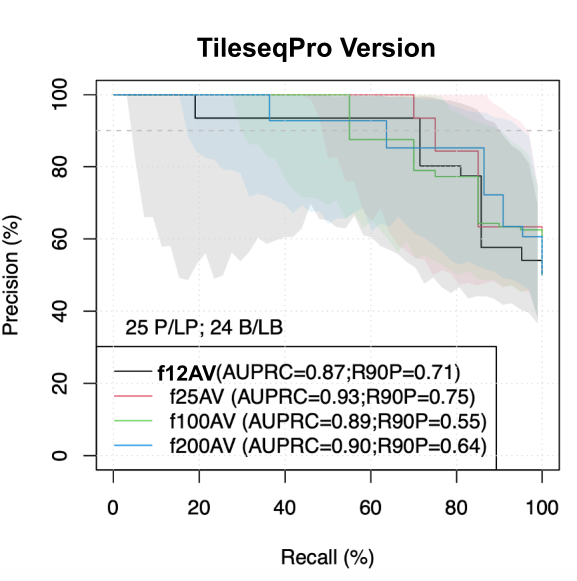
\includegraphics[width=.45\textwidth]{Figures/MTHFR/new_PRC.png} }}%
    \qquad
    \subfloat[\centering 2021 version PRC]{{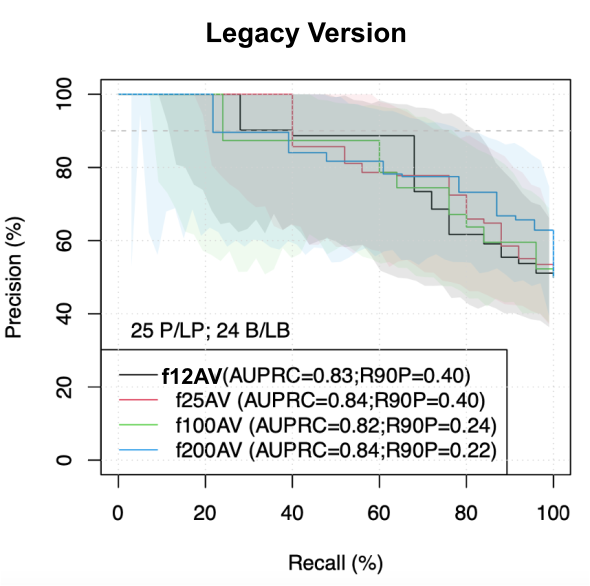
\includegraphics[width=.45\textwidth]{Figures/MTHFR/old_PRC.png} }}%
    \caption{PRC for 2023 and 2021 version of MTHFR maps in A222V background, compared between different folate concentrations(map: f12AV, f25AV, f100AV, f200AV) using the manually curated reference sets from Weile et al.\cite{weile_shifting_2021}}%
    \label{fig:PRC MTHFR in A222V Background}%
\end{figure}

The transformation to log-likelihood ratio for TileseqPro MTHFR maps at different folate concentrations are compared in Figure \ref{fig:LLR MTHFR}. The overall shapes of these LLR curves are similar despite some minor differences, where LLR is positive when the fitness scores range from -0.5 to 0.5, indicate a tendency towards pathogenicity. Whereas LLR is negative when the fitness score is approximately between 0.8 to 1.5. There is still issues with the transformation function, since in the f200AV map the negative LLR spikes at fitness scores above 1.5 with no real reference data. 

% LLR?
\begin{figure}[H]%
    \centering
    \subfloat[\centering f12AV]{{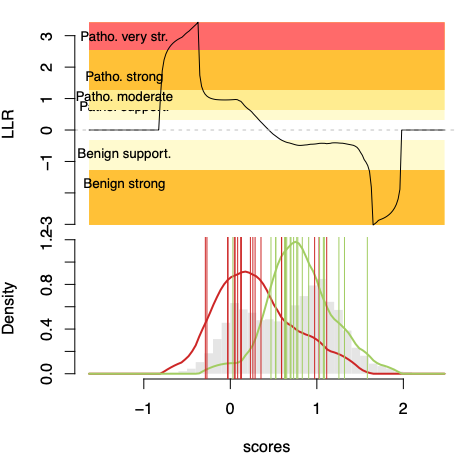
\includegraphics[width=.45\textwidth]{Figures/MTHFR/f12AV_LLR.png} }}%
    \qquad
    \subfloat[\centering f25AV]{{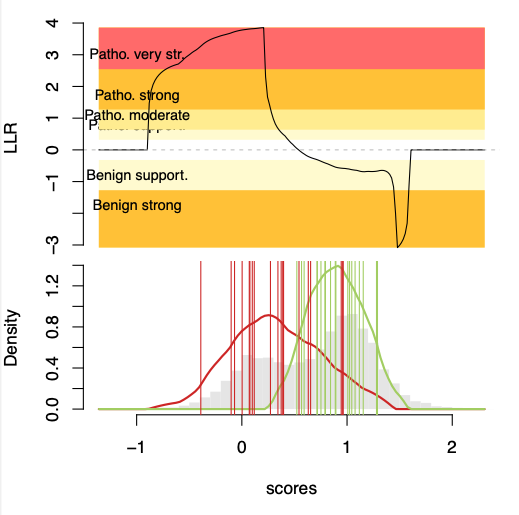
\includegraphics[width=.45\textwidth]{Figures/MTHFR/f25AV_LLR.png} }}%
    \qquad
    \subfloat[\centering f100AV]{{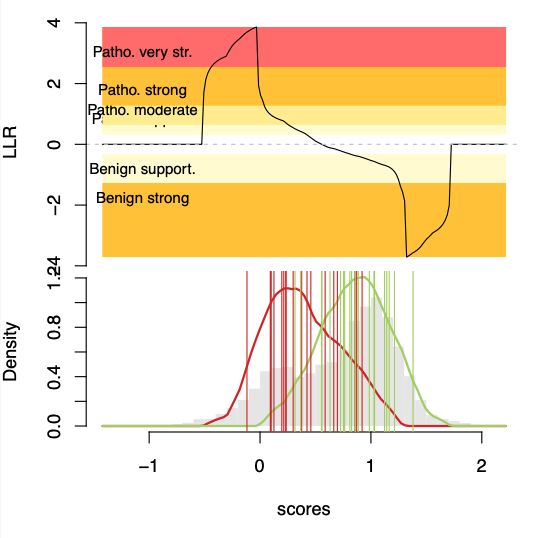
\includegraphics[width=.45\textwidth]{Figures/MTHFR/f100AV_LLR.png} }}%
    \qquad
    \subfloat[\centering f200AV]{{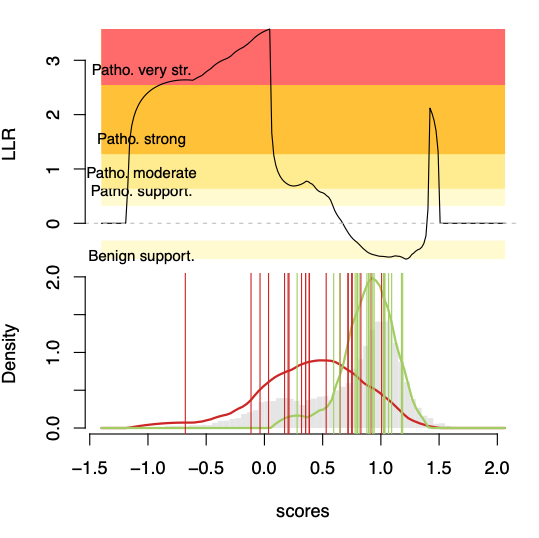
\includegraphics[width=.45\textwidth]{Figures/MTHFR/f200AV_LLR.png} }}%
    \caption{LLR of pathogenicity of MTHFR variants in A222V background, separated by different folate concentrations.}%
    \label{fig:LLR MTHFR}%
\end{figure}


\subsubsection{Conclusion}
The TileseqPro version of MTHFR maps outperformed our Legacy version in terms of getting more precision in classifying variants. However, the fitness scores calculated by the Legacy and TileseqPro pipelines need to be compared again after finding the non-flipped and floored scores. 




\newpage
\section{Discussion}
In this BCB330 Project, we successfully re-processed the variant effect maps for several genes using the TileseqPro pipelines. We evaluated their performance by inspecting QC results, comparing fitness scores with the Legacy pipelines, finding the moving window correlation to computational predictor VARITY, and drawing the PRC. We also inferred the fitness score ranges that corresponding to "benign" and "pathogenic" by calculating Log-likelihood of pathogenicity. 

The TileseqPro and the Legacy pipeline performed similarly in SUMO1 map, but TileseqPro outperformed the Legacy pipelines in CALM1 map however at the expense of losing much of its original coverage, since we filtered out a lot more low quality data than before. To address this problem, machine-learning methods could be applied to impute those "missing spots" in the next step. For the MTHFR map in A222V background, TileseqPro pipelines performed better in getting more precision in prediction, but the fitness scores calculated by the TileseqPro and Legacy pipelines need to be compared after re-scaling them. 

Other future goals for this project are as follows: First, we will continue to re-processing more of the existing maps on MaveDB, compare the results with the older version, and give recommendation on optimizing the pipeline implementations. Second, we will try curating benchmark reference sets for disease genes, when there is no good reference available for them. Third, we will continue to document the results for the maps that we already re-processed
% including GDI1, TECR, UBE2I 
to a GitHub wiki page. Furthermore, we will also compare the new and old fitness scores of disease genes to other computational predictors such as ESM1v\cite{lin2023evolutionary} and PROVEAN\cite{sandell_fitness_2022}.


\section{Supplementary Materials}
Supplementary Materials can be found on GitHub at \href{https://github.com/Bilin22/BCB330-Final-Report/blob/main/main/Supplementary.pdf}{Supplementary}


\bibliographystyle{unsrt}
\bibliography{reference}

\end{document}